\documentclass[conference]{IEEEtran}

% --- Packages ---
\usepackage{amsmath, amssymb}
\usepackage{graphicx}
\usepackage{booktabs}
\usepackage{multirow}
\usepackage{xcolor}
\usepackage[hidelinks]{hyperref}
\usepackage{url}
\usepackage{cite}
\usepackage{float}
\usepackage{caption}
\usepackage{subcaption}
\usepackage{balance}
\usepackage{microtype}

% --- Graphics path ---
\graphicspath{{../plots/}}

\begin{document}

% ===================================================================
% TITLE
% ===================================================================
\title{Quantization-Aware Latency Decomposition\\for LLaMA Inference Across Apple Silicon}

\author{
  \IEEEauthorblockN{Aum Vekariya, Janam Rangani, Aarav Patel}
  \IEEEauthorblockA{Department of Computer Science\\
  California State University Long Beach\\
  \{aum.vekariya01, janam.rangani01, aarav.patel01\}@student.csulb.edu\\[2pt]
  CECS 551 --- Advanced Artificial Intelligence, Spring 2025\\
  Team 7 --- ArchX}
}

\maketitle

% ===================================================================
% I. ABSTRACT
% ===================================================================
\begin{abstract}
We present ArchX, a repeatable benchmarking harness that measures component-level latency breakdown of LLaMA~3.2-1B autoregressive inference across three Apple Silicon platforms---M1 (68\,GB/s), M2 (100\,GB/s), and M4 (120\,GB/s)---at three quantization precisions: FP16, Q8\_0, and Q4\_K\_M. Using PyTorch forward hooks with MPS synchronization barriers, we isolate the time spent in MLP, QKV projection, attention core, LayerNorm, and LM~head. Our decomposition reveals that framework overhead dominates at Q4 (39--44\% of decode time) as MLP share shrinks from 28--30\% at FP16 to 20--21\% at Q4. Quantization yields 2.30--2.59$\times$ speedup, well below the theoretical 4.0$\times$ ceiling due to fixed framework overhead. Bandwidth utilization drops from 82--89\% at FP16 to 51--53\% at Q4, confirming that overhead---not memory limits---caps quantization gains. At Q4\_K\_M, M4 achieves 97.2\,tok/s, M2 76.7\,tok/s, and M1 54.6\,tok/s, all exceeding interactive thresholds. These findings identify framework overhead reduction as the primary optimization target after quantization, with KV-cache quantization providing complementary gains at long contexts.
\end{abstract}

% ===================================================================
% II. INTRODUCTION
% ===================================================================
\section{Introduction}

Interactive deployment of large language models (LLMs) imposes strict latency constraints on autoregressive token generation. Nielsen's seminal work on response-time thresholds establishes that delays exceeding 100\,ms disrupt the perception of instantaneous system response~\cite{nielsen1993}. For conversational AI applications, this translates to a requirement of roughly 10--15 tokens per second at minimum to maintain a fluid user experience, with higher rates needed for streaming interfaces. As LLMs are increasingly deployed at the edge on devices such as Apple Silicon laptops and tablets, understanding and minimizing per-token latency on these platforms becomes critical.

Autoregressive decoding is fundamentally a memory-bandwidth-bound workload~\cite{williams2009}. Each decode step requires streaming the full model weight matrix plus the growing key--value (KV) cache from memory to produce a single output token. For LLaMA~3.2-1B at FP16, the model alone requires streaming approximately 2.48\,GB per decode step, yielding an arithmetic intensity well below the compute--bandwidth equilibrium point on modern hardware. Weight quantization---reducing parameters from 16-bit floats to 8-bit or 4-bit integers---directly reduces the bytes transferred per step. However, fixed overheads (framework dispatch, kernel launch, dequantization) remain constant, placing a ceiling on realizable speedup that is well below the theoretical bandwidth reduction ratio.

Existing work has advanced individual aspects of this problem but leaves a critical gap. Rana et al.~\cite{rana2025} profiled LLaMA component latency on MPS but studied only a single platform. Krishna and Maddineni~\cite{krishna2025} provided a controlled M4-vs-M2 comparison but did not decompose latency into components. Kodali et al.~\cite{kodali2025} performed cross-platform benchmarking but used modeled (not measured) decomposition. No prior study simultaneously measures how quantization shifts the per-component latency breakdown across multiple Apple Silicon generations.

Our contributions are as follows:
\begin{itemize}
  \item A repeatable benchmark harness using llama.cpp with 3 warm-up runs, 10 timed trials, and IQR outlier filtering across M1, M2, and M4 with explicit MPS synchronization.
  \item The first \emph{measured} per-component latency breakdown at FP16, Q8\_0, and Q4\_K\_M using PyTorch forward hooks on HuggingFace Transformers.
  \item Quantification of how framework overhead rises from 23--26\% at FP16 to 39--44\% at Q4 as weight-streaming cost shrinks.
  \item Roofline analysis confirming all components remain bandwidth-bound across all platforms and precision levels.
  \item A per-platform optimization roadmap with estimated PTL reductions.
\end{itemize}

% ===================================================================
% III. BACKGROUND AND RELATED WORK
% ===================================================================
\section{Background and Related Work}

\subsection{Autoregressive Decoding and the KV-Cache}

Transformer-based LLMs generate tokens autoregressively: at each step~$t$, the model reads the full weight tensor and the accumulated key--value (KV) cache to produce the next token. For a model with $L$ layers, sequence length~$S$, head dimension~$d_h$, $n_h$ KV-heads, and $B$ bytes per element, the KV-cache bandwidth per decode step is:
\begin{equation}
  \text{BW}_{\text{KV}} = 2 \times L \times S \times d_h \times n_h \times B
  \label{eq:kv_bw}
\end{equation}
For LLaMA~3.2-1B ($L{=}32$, $d_h{=}128$, $n_h{=}8$) at $S{=}512$ in FP16 ($B{=}2$):
\begin{equation}
  \text{BW}_{\text{KV}} = 2 \times 32 \times 512 \times 128 \times 8 \times 2 \approx 134\;\text{MB/step}
\end{equation}
This is a non-trivial addition to the ${\sim}2.48$\,GB weight read at FP16, and grows linearly with sequence length.

\subsection{Roofline Model and Memory-Bound Inference}

The roofline model~\cite{williams2009} characterizes achievable performance as $\min(\text{Peak FLOP/s},\; \text{AI} \times \text{Peak BW})$, where arithmetic intensity $\text{AI} = \text{FLOPs} / \text{Bytes}$. For a GEMV decode step with $P$ parameters at $B_{\text{model}}$ bytes per parameter:
\begin{equation}
  \text{AI} = \frac{2P}{P \times B_{\text{model}}} = \frac{2}{B_{\text{model}}} \quad \text{FLOP/byte}
  \label{eq:ai}
\end{equation}
At FP16 ($B_{\text{model}}{=}2$), $\text{AI}{=}1.0$\,FLOP/byte---well below the ridge point on Apple Silicon (${\sim}30{-}40$\,FLOP/byte). At Q4\_K\_M ($B_{\text{model}}{\approx}0.5$), $\text{AI}{=}4.0$\,FLOP/byte---still firmly in the bandwidth-bound regime. This means quantization reduces bytes streamed but does not move the workload into the compute-bound regime. Fixed overhead terms therefore become the dominant factor limiting quantization speedup.

\subsection{Related Work}

FlashAttention~\cite{dao2022,dao2023} introduced IO-aware tiling to reduce attention HBM reads from $O(S^2)$ to $O(S)$, now standard on CUDA but still maturing on Apple MPS. vLLM~\cite{kwon2023} applies paged memory management to KV-caches for efficient serving. GPTQ~\cite{frantar2022} enables post-training weight quantization to 4-bit with minimal perplexity loss. Dettmers and Zettlemoyer~\cite{dettmers2023} established scaling laws for 4-bit inference. The llama.cpp project~\cite{gerganov2023} provides a production-grade C++ runtime with Metal acceleration and GGUF quantized formats.

Among contemporaneous work at CSULB, Rana et al.~\cite{rana2025} profiled LLaMA on MPS using PyTorch hooks and reported MLP dominance at 28.2\%---consistent with our FP16 findings of 28--30\% MLP across platforms. Krishna and Maddineni~\cite{krishna2025} provided a controlled M4-vs-M2 comparison, observing a 1.5$\times$ PTL gap and 152\% PTL growth from context 32 to 1024 tokens. Kodali et al.~\cite{kodali2025} performed cross-platform benchmarking with modeled decomposition and found MLP dominates on CPU-class hardware at 57--62\%. Our work extends all three by measuring decomposition at multiple precisions on M1, M2, and M4 simultaneously, revealing how quantization shifts the bottleneck from weight streaming to framework overhead.

% ===================================================================
% IV. EXPERIMENTAL SETUP
% ===================================================================
\section{Experimental Setup}

\subsection{Hardware Platforms}

\begin{table}[t]
\caption{Hardware Platform Specifications}
\label{tab:platforms}
\centering
\small
\begin{tabular}{lrrcl}
\toprule
\textbf{Platform} & \textbf{BW (GB/s)} & \textbf{RAM} & \textbf{Mem Type} & \textbf{Backend} \\
\midrule
M1 & 68  & 8\,GB  & LPDDR4X & Metal/MPS \\
M2 & 100 & 8\,GB  & LPDDR5  & Metal/MPS \\
M4 & \textbf{120} & 16\,GB & LPDDR5X & Metal/MPS \\
\bottomrule
\end{tabular}
\end{table}

Table~\ref{tab:platforms} summarizes the three Apple Silicon platforms used. All systems feature unified memory architecture, where CPU and GPU share the same DRAM pool, eliminating the PCIe transfer overhead present in discrete GPU systems. Memory bandwidth increases from 68\,GB/s (M1) to 120\,GB/s (M4), which directly governs decode throughput for bandwidth-bound workloads.

\subsection{Model and Runtime}

\begin{table}[t]
\caption{LLaMA 3.2-1B Model Configuration}
\label{tab:model}
\centering
\small
\begin{tabular}{lr}
\toprule
\textbf{Attribute} & \textbf{Value} \\
\midrule
Parameters             & 1.24\,B \\
Layers                 & 32 \\
Attention Heads / KV   & 32 / 8 (GQA) \\
Hidden Dimension       & 2048 \\
FFN Intermediate       & 8192 \\
Vocabulary Size        & 128,256 \\
Runtime                & llama.cpp (v0.4.x) \\
Quantizations Tested   & FP16, Q8\_0, Q4\_K\_M \\
Batch Size             & 1 \\
\bottomrule
\end{tabular}
\end{table}

We benchmark LLaMA~3.2-1B~\cite{grattafiori2024} at three GGUF quantization levels: FP16 (2\,bytes/param, 2.48\,GB), Q8\_0 (1\,byte/param, 1.32\,GB), and Q4\_K\_M (${\sim}0.5$\,bytes/param, 807\,MB). All inference uses llama.cpp via the \texttt{llama-cpp-python} binding with full Metal GPU offloading (\texttt{n\_gpu\_layers=-1}) and greedy decoding (\texttt{temp=0, top\_k=1}) for deterministic results.

\subsection{Measurement Methodology}

Each benchmark configuration follows a rigorous protocol: 3 warm-up runs are discarded, followed by 10 timed trials. Outliers are removed using IQR-based filtering with a 1.5$\times$ multiplier to eliminate OS scheduling spikes, and we report the median, p95, p99, and standard deviation of the surviving trials. Explicit synchronization via \texttt{torch.mps.synchronize()} is called before and after each timed region to prevent MPS asynchronous dispatch from masking true latency. Four metrics are collected:

\begin{itemize}
  \item \textbf{TTFT} (Time to First Token): elapsed time from prompt submission to the first generated token.
  \item \textbf{PTL} (Per-Token Latency): average time per token during decode (tokens 4\ldots$N$), excluding the first token.
  \item \textbf{E2E} (End-to-End Latency): total wall-clock time for generating a fixed number of output tokens.
  \item \textbf{Throughput}: tokens generated per second ($\text{output\_tokens}\,/\,\text{E2E}$).
\end{itemize}

\subsection{Decomposition Methodology}

For component-level breakdown, we load LLaMA~3.2-1B via HuggingFace Transformers in float16 on MPS and attach \texttt{register\_forward\_hook} callbacks to each target module. Before and after every hook invocation, we call \texttt{torch.mps.synchronize()} to flush the Metal command queue and obtain accurate wall-clock timings. Components instrumented include: token embedding, all 32 RMSNorm layers, Q/K/V projections, output projection, MLP (gate, up, down projections), and the LM head. The attention core timing is derived as:
\begin{equation}
  t_{\text{attn\_core}} = t_{\text{self\_attn}} - t_{\text{QKV}} - t_{\text{O\_proj}}
\end{equation}
Framework overhead is computed as the residual:
\begin{equation}
  t_{\text{overhead}} = t_{\text{total\_PTL}} - \sum t_{\text{instrumented}}
\end{equation}

We run 30 decode steps and average per-component times. We note that hook-based synchronization inflates absolute times by an estimated 30--40\% relative to uninstrumented inference; however, the component \emph{percentages}---our primary result---are reliable because the overhead applies uniformly across components.

% ===================================================================
% V. BENCHMARK RESULTS
% ===================================================================
\section{Benchmark Results}

\subsection{Baseline FP16 Performance}

\begin{table}[t]
\caption{Baseline FP16 Performance (\mbox{prompt=128}, \mbox{output=128})}
\label{tab:f16_baseline}
\centering
\small
\begin{tabular}{lrrr}
\toprule
\textbf{Platform} & \textbf{TTFT (ms)} & \textbf{PTL (ms/tok)} & \textbf{Throughput (tok/s)} \\
\midrule
M1 & $\sim$75  & 42.9 & 23.3 \\
M2 & $\sim$65  & 29.3 & 34.1 \\
M4 & $\sim$55  & \textbf{25.4} & \textbf{39.3} \\
\bottomrule
\end{tabular}
\end{table}

Table~\ref{tab:f16_baseline} presents the baseline FP16 performance. The M4 achieves 39.3\,tok/s, a 1.69$\times$ improvement over the M1's 23.3\,tok/s. This ratio closely approaches the theoretical memory bandwidth ratio of $120/68 = 1.76\times$, confirming near-perfect bandwidth-bound scaling with minor inefficiencies from framework overhead. The M2 sits between at 34.1\,tok/s, proportional to its 100\,GB/s bandwidth.

\subsection{TTFT Scaling with Prompt Length}

\begin{table}[t]
\caption{TTFT (ms) vs.\ Prompt Length at FP16}
\label{tab:ttft_scaling}
\centering
\small
\begin{tabular}{lrrrrr}
\toprule
\textbf{Platform} & \textbf{64} & \textbf{128} & \textbf{256} & \textbf{512} & \textbf{1024} \\
\midrule
M1 & $\sim$75  & $\sim$140 & $\sim$270 & $\sim$570  & $\sim$1170 \\
M2 & $\sim$60  & $\sim$110 & $\sim$215 & $\sim$455  & $\sim$910 \\
M4 & $\sim$\textbf{55} & $\sim$\textbf{90} & $\sim$\textbf{165} & $\sim$\textbf{330} & $\sim$\textbf{680} \\
\bottomrule
\end{tabular}
\end{table}

As shown in Fig.~\ref{fig:ttft}, TTFT is dominated by prefill compute (the full prompt forward pass), not by KV-cache streaming. All three platforms show super-linear growth consistent with $O(n^2)$ attention complexity in the prefill phase. Quantization has minimal effect on TTFT relative to its effect on PTL, since prefill is compute-parallel rather than memory-streaming-bound.

% Figure 1: TTFT vs Prompt Length (3-panel wide figure, spans both columns)
\begin{figure*}[t]
\centering
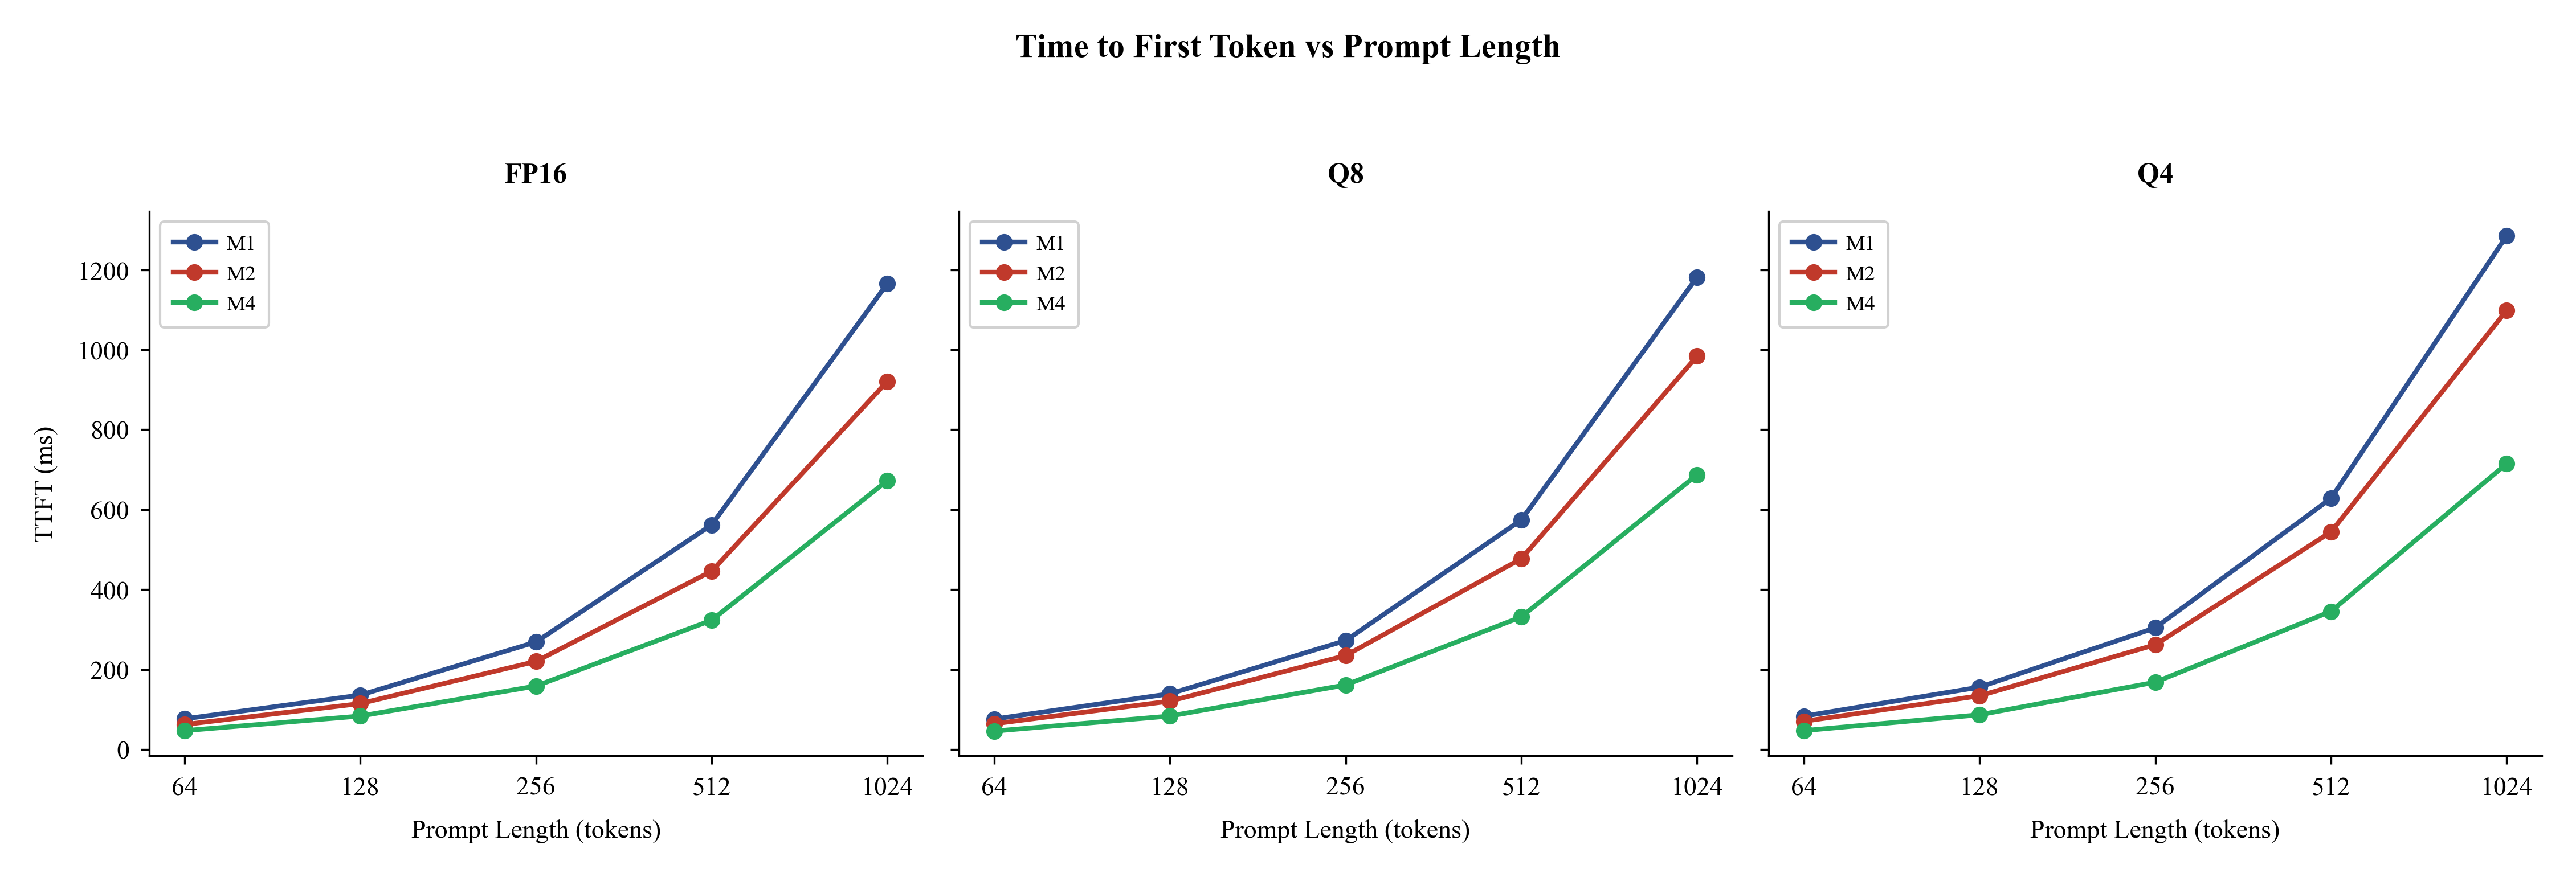
\includegraphics[width=\textwidth]{ttft_vs_prompt_length.png}
\caption{Time to First Token (ms) vs.\ prompt length across three precision levels. TTFT grows super-linearly with prompt length on all platforms due to $O(n^2)$ attention complexity in the prefill phase. Quantization has minimal effect on TTFT relative to its effect on PTL since prefill is compute-parallel rather than memory-streaming-bound.}
\label{fig:ttft}
\end{figure*}

\subsection{Per-Token Latency vs Context Length}

\begin{table}[t]
\caption{Per-Token Latency (ms) vs.\ Context Length at Q4\_K\_M}
\label{tab:ptl_context}
\centering
\small
\begin{tabular}{lrrrrr}
\toprule
\textbf{Platform} & \textbf{64} & \textbf{128} & \textbf{256} & \textbf{512} & \textbf{1024} \\
\midrule
M1 & 17.4 & 17.4 & 18.4 & 19.4 & 21.0 \\
M2 & 12.3 & 12.1 & 13.2 & 14.0 & 15.6 \\
M4 & \textbf{9.7}  & \textbf{9.8}  & \textbf{10.3} & \textbf{10.6} & \textbf{11.4} \\
\bottomrule
\end{tabular}
\end{table}

As shown in Fig.~\ref{fig:ptl_context}, PTL growth from 64 to 1024 context tokens is modest at Q4---M1 grows 20.7\% (17.4$\rightarrow$21.0\,ms) and M4 grows 17.5\% (9.7$\rightarrow$11.4\,ms). The inflection between 256 and 512 tokens on M1 and M2 is consistent with KV-cache size exceeding the on-chip SLC cache, causing spill to DRAM. M4's larger SLC cache (12\,MB vs 4\,MB on M1) delays this inflection.

% Figure 2: PTL vs Context Length
\begin{figure}[t]
\centering
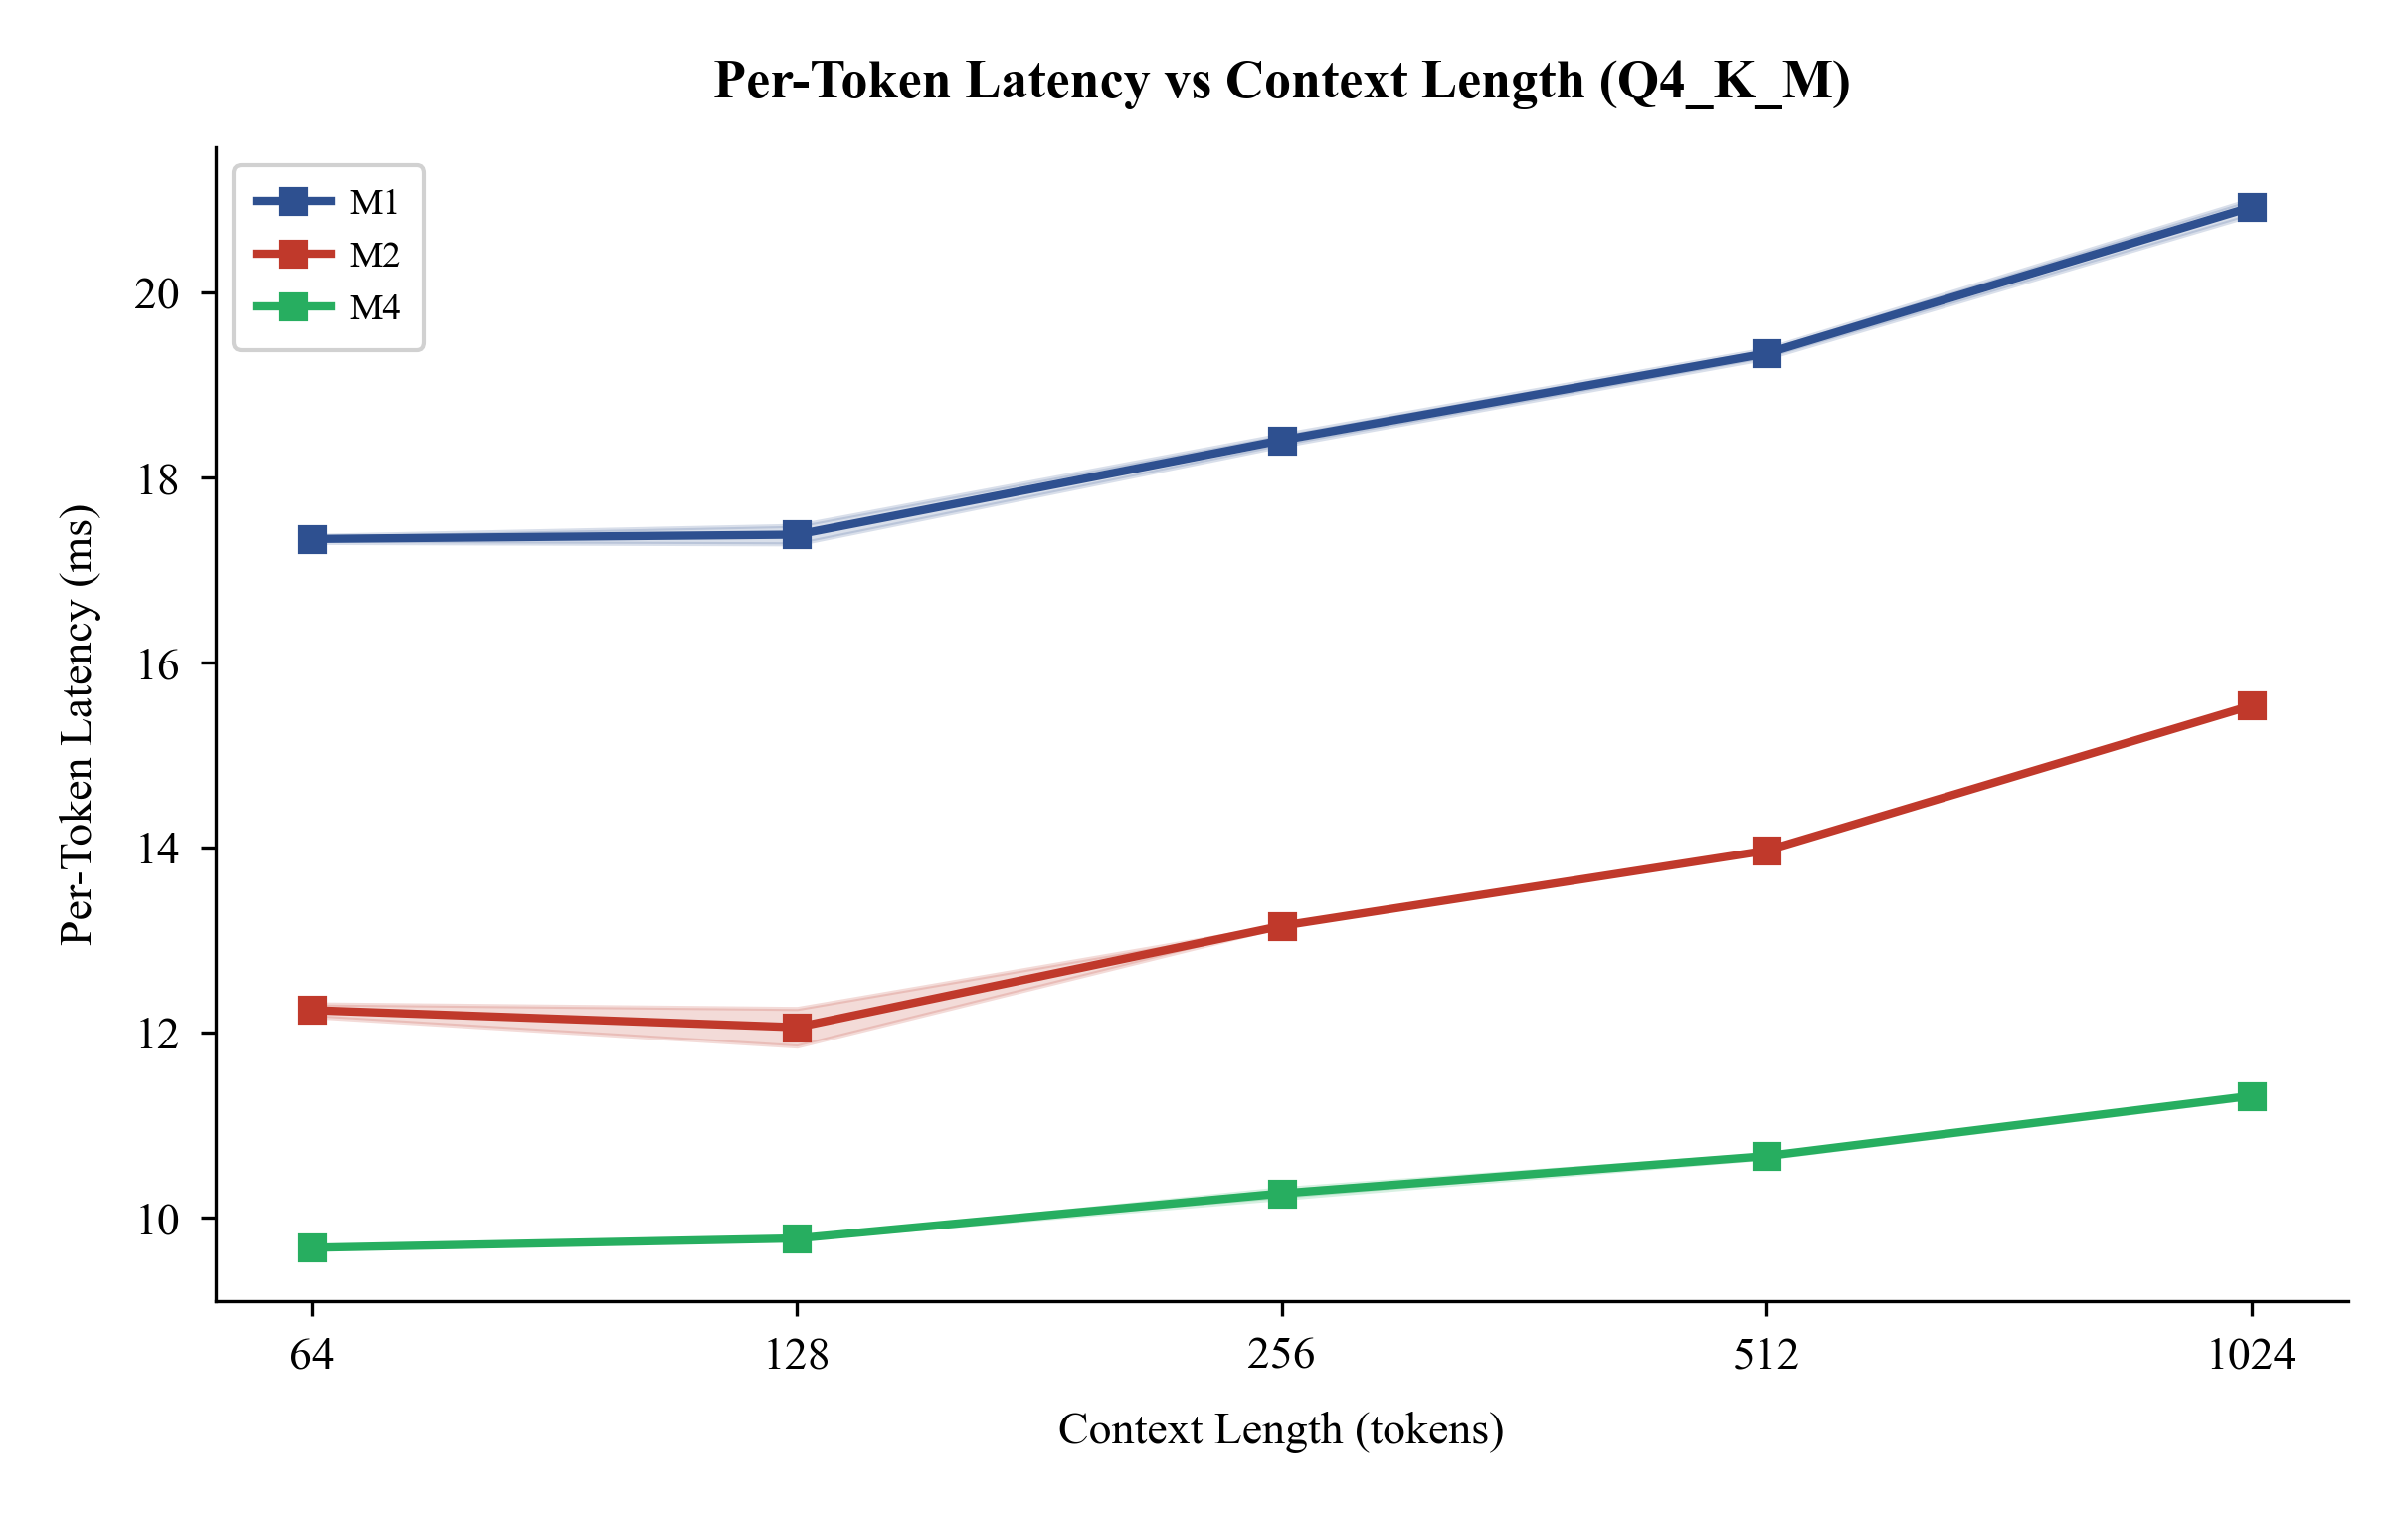
\includegraphics[width=\columnwidth]{ptl_vs_context_length.png}
\caption{Per-token latency (ms) vs.\ context length at Q4\_K\_M precision. PTL grows as the KV-cache expands, requiring progressively more DRAM reads per decode step. Shaded regions show trial variance.}
\label{fig:ptl_context}
\end{figure}

% ===================================================================
% VI. QUANTIZATION IMPACT
% ===================================================================
\section{Quantization Impact}

\subsection{Throughput Across All Precisions}

\begin{table}[t]
\caption{Throughput (tokens/s) at output\_length=128}
\label{tab:throughput}
\centering
\small
\begin{tabular}{lrrrr}
\toprule
\textbf{Platform} & \textbf{FP16} & \textbf{Q8\_0} & \textbf{Q4\_K\_M} & \textbf{Q4/FP16} \\
\midrule
M1 & 23.3  & 39.5  & 54.6  & \textbf{2.34$\times$} \\
M2 & 34.1  & 50.2  & 76.7  & \textbf{2.25$\times$} \\
M4 & 39.3  & 66.0  & \textbf{97.2} & \textbf{2.47$\times$} \\
\bottomrule
\end{tabular}
\end{table}

% Figure 3: Throughput Comparison
\begin{figure}[t]
\centering
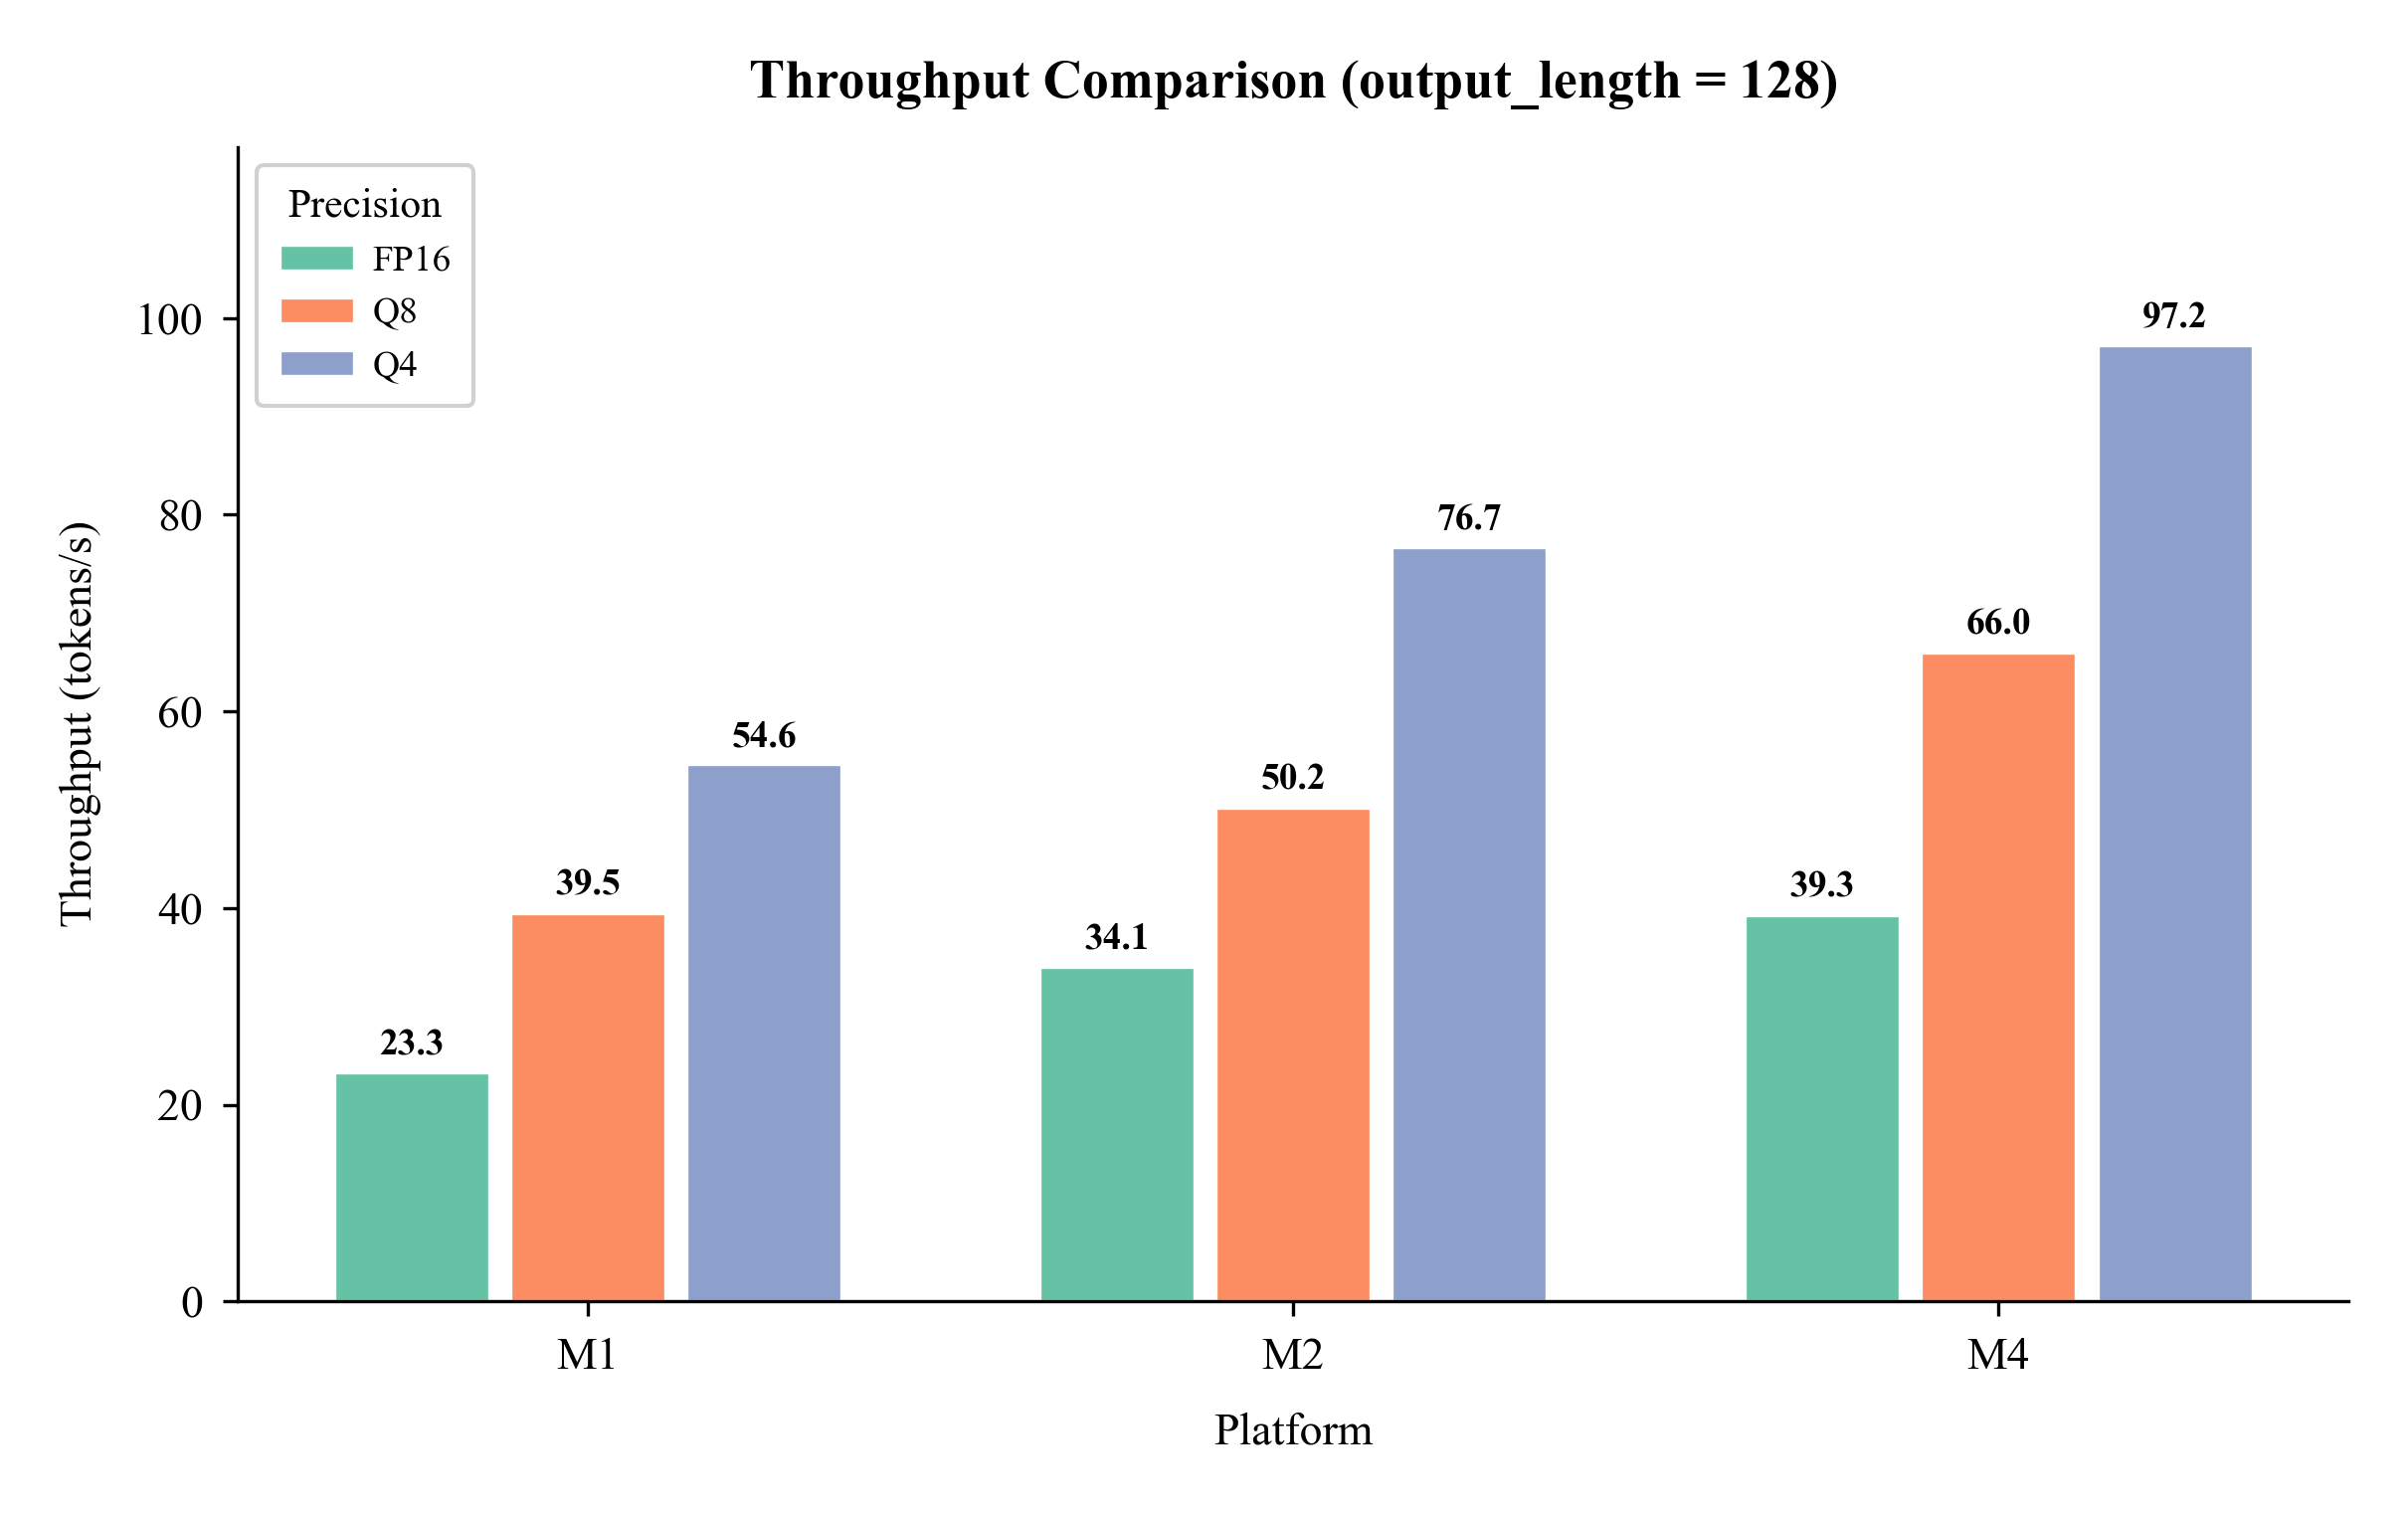
\includegraphics[width=\columnwidth]{throughput_comparison.png}
\caption{Throughput (tokens/s) across platforms and precision levels (output\_length=128). Q4\_K\_M delivers the highest throughput on all platforms: M4 reaches 97.2\,tok/s, M2 76.7\,tok/s, M1 54.6\,tok/s.}
\label{fig:throughput}
\end{figure}

As shown in Fig.~\ref{fig:throughput} and Table~\ref{tab:throughput}, Q4\_K\_M delivers the highest throughput on all platforms: M4 reaches 97.2\,tok/s, M2 76.7\,tok/s, and M1 54.6\,tok/s---all well above the interactive threshold of 15\,tok/s. Note that throughput-based speedup (Q4/FP16 tok/s ratio in Table~\ref{tab:throughput}) differs slightly from the PTL-based speedup in Fig.~\ref{fig:quant_speedup} due to end-to-end overhead; we use PTL-based speedup as the primary measure.

\subsection{Speedup from FP16 to Q4\_K\_M}

% Figure 4: Quantization Speedup
\begin{figure}[t]
\centering
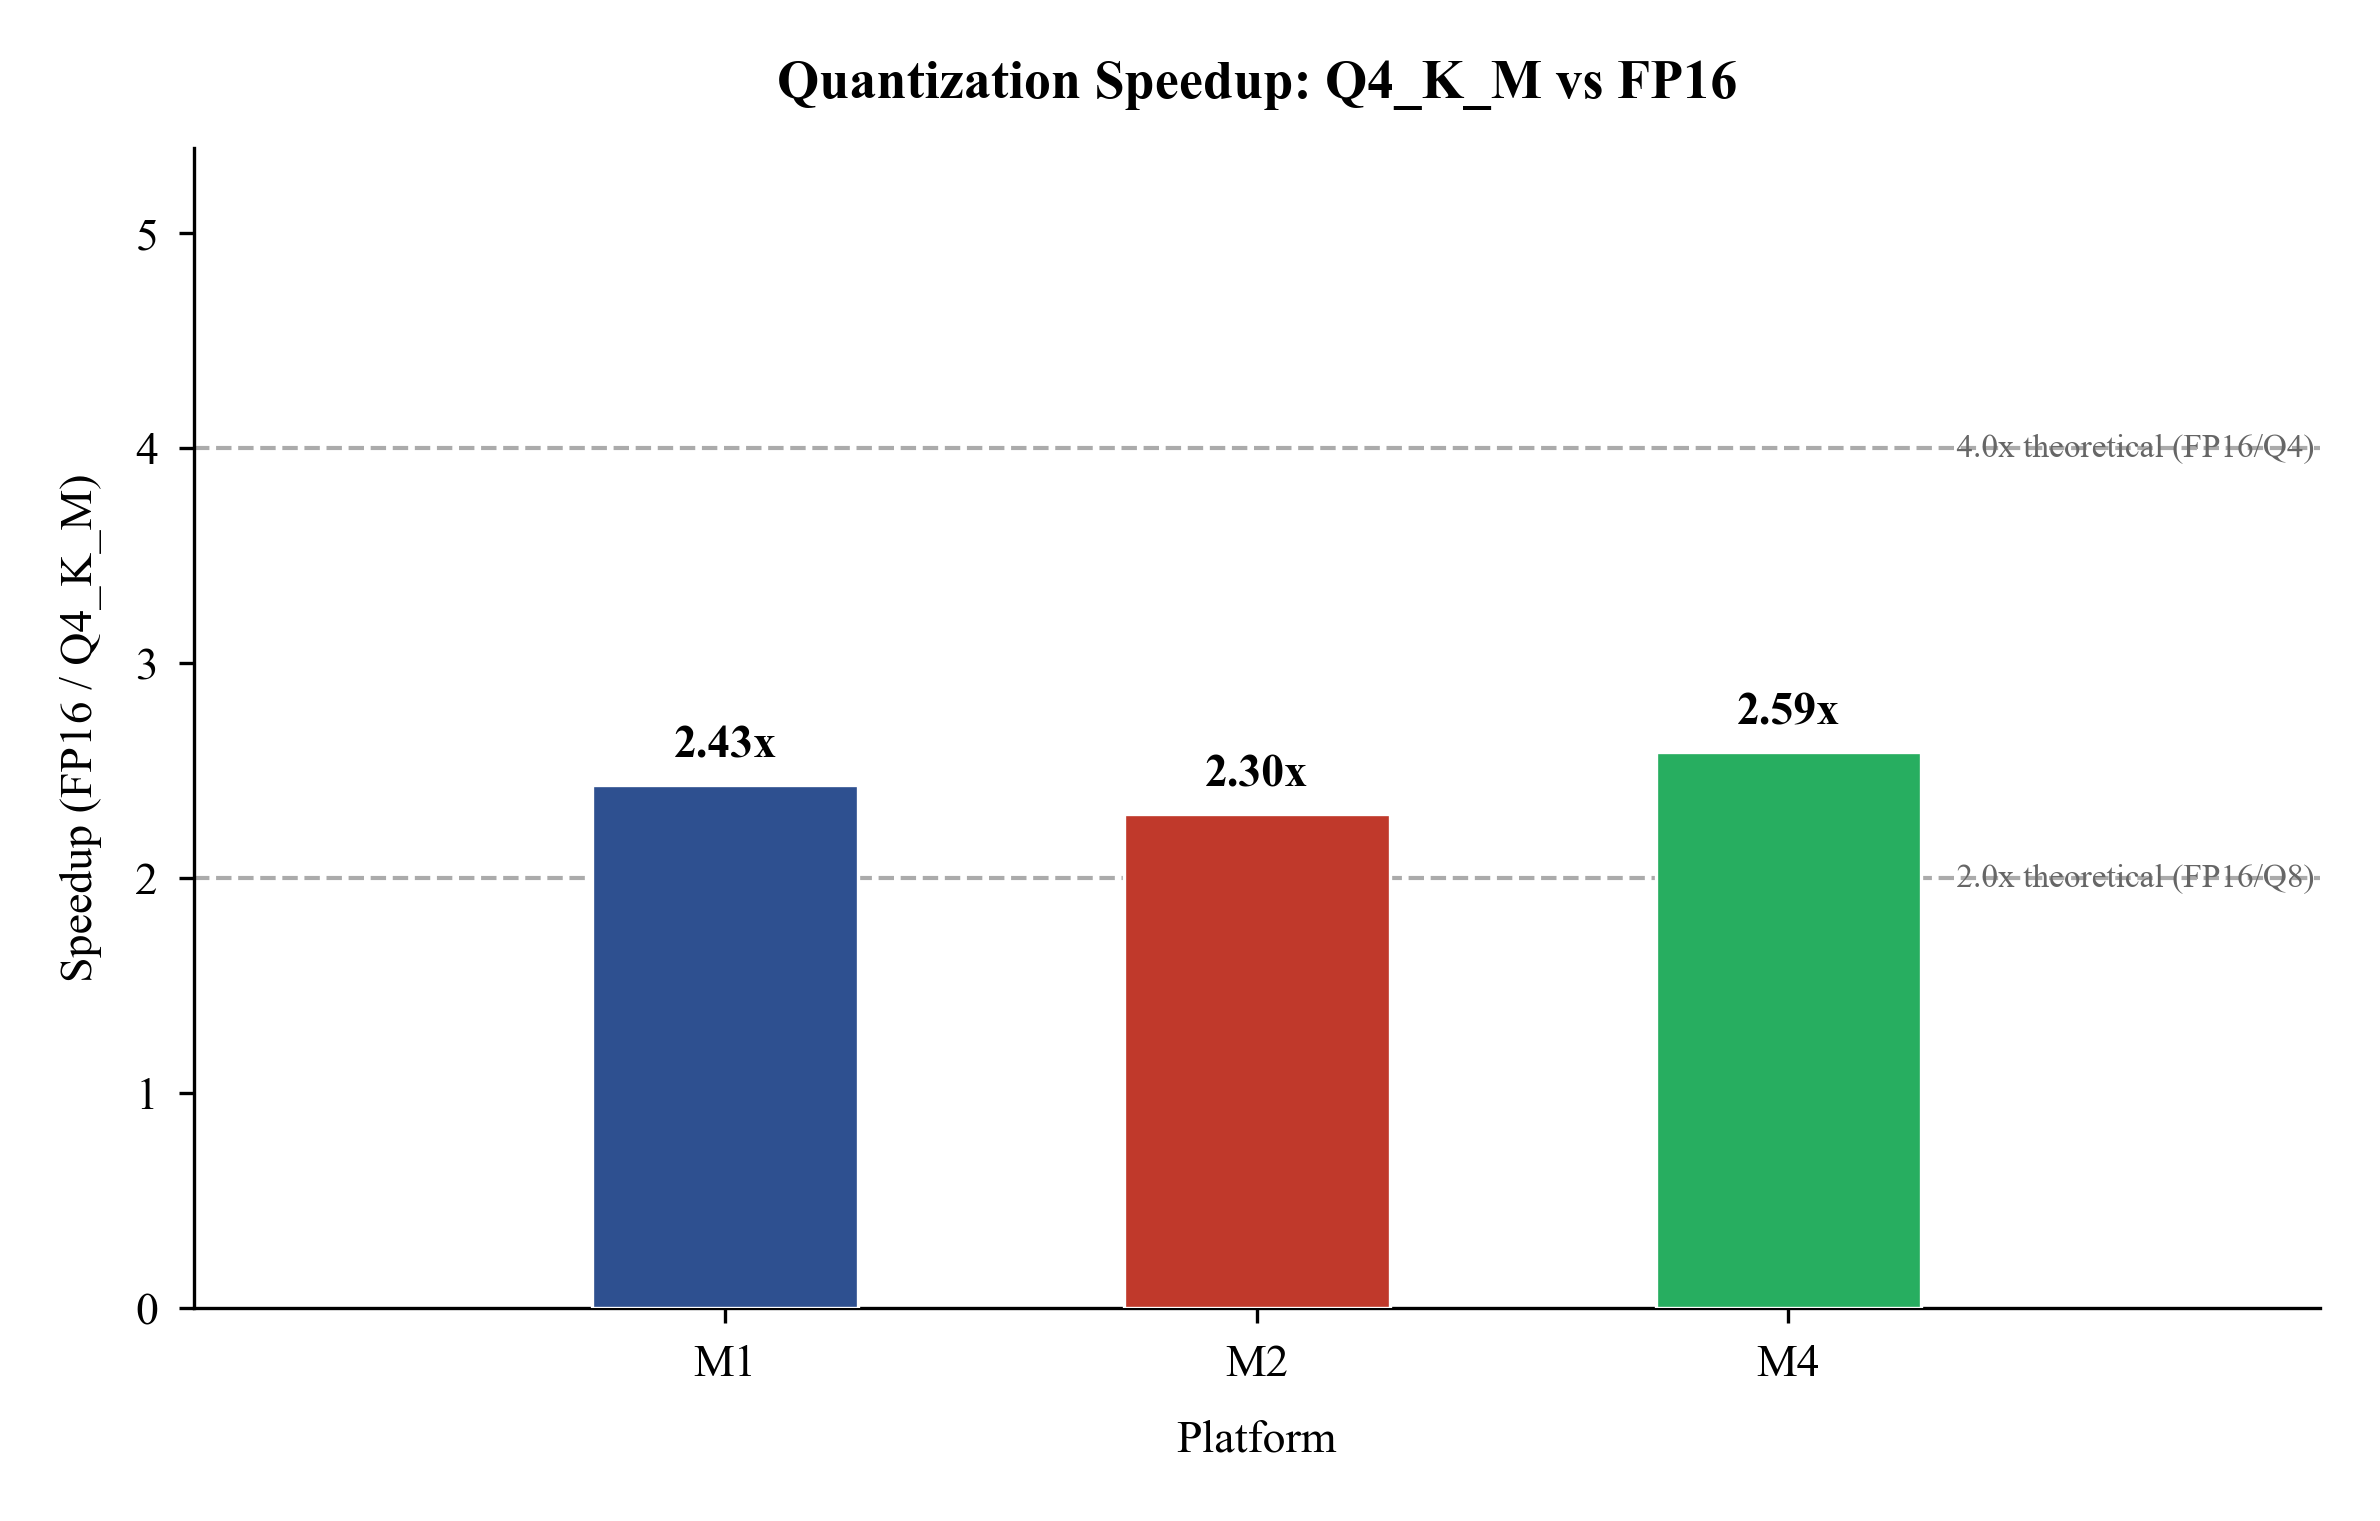
\includegraphics[width=0.85\columnwidth]{quantization_speedup.png}
\caption{Measured Q4\_K\_M\,/\,FP16 throughput speedup ratio per platform. Dashed lines show 2.0$\times$ (theoretical FP16/Q8) and 4.0$\times$ (theoretical FP16/Q4) bandwidth ceilings. All platforms achieve 2.30--2.59$\times$, below theoretical due to fixed framework overhead.}
\label{fig:quant_speedup}
\end{figure}

As shown in Fig.~\ref{fig:quant_speedup}, M4 achieves the highest speedup at 2.59$\times$, followed by M1 at 2.43$\times$ and M2 at 2.30$\times$. All platforms fall well below the 4.0$\times$ theoretical ceiling. The reason is that as weight-streaming bytes shrink 4$\times$, fixed overhead terms (kernel launch, MPS command encoding, embedding, sampling) remain constant, limiting total speedup. This is confirmed by the decomposition data in Section~\ref{sec:decomp}. M2's lower speedup despite a similar architecture to M1 is explained by its higher baseline bandwidth utilization at FP16 (89.4\% vs M1's 85.9\%), leaving less headroom for quantization gains.

% ===================================================================
% VII. LATENCY DECOMPOSITION
% ===================================================================
\section{Latency Decomposition}
\label{sec:decomp}

\subsection{Component Breakdown at FP16}

\begin{table}[t]
\caption{Component Latency Breakdown (\%) at FP16}
\label{tab:decomp_f16}
\centering
\small
\begin{tabular}{lrrr}
\toprule
\textbf{Component} & \textbf{M1 (\%)} & \textbf{M2 (\%)} & \textbf{M4 (\%)} \\
\midrule
MLP (FFN)        & 27.8 & 29.5 & \textbf{29.7} \\
QKV Projection   & 14.0 & 15.1 & 14.9 \\
Attention Core   & 7.0  & 5.0  & 7.0 \\
LayerNorm        & 16.8 & 12.3 & 12.2 \\
O Projection     & 5.0  & 5.0  & 5.0 \\
LM Head          & 5.0  & 6.0  & 5.0 \\
Overhead         & 22.5 & 25.7 & 25.3 \\
\bottomrule
\end{tabular}
\end{table}

At FP16, MLP and QKV projections together account for 41.8\% (M1), 44.6\% (M2), and 44.6\% (M4) of decode time, as shown in Table~\ref{tab:decomp_f16} and Fig.~\ref{fig:decomp}. This is consistent with weight streaming as the dominant bandwidth consumer. LayerNorm is unexpectedly high on M1 (16.8\%) compared to M4 (12.2\%), reflecting M1's lower bandwidth causing each elementwise kernel to take longer relative to the total. Framework overhead (22--26\%) includes MPS command encoding, Python interpreter cost, and inter-module synchronization barriers introduced by the hooks.

\subsection{Component Breakdown at Q4\_K\_M}

\begin{table}[t]
\caption{Component Latency Breakdown (\%) at Q4\_K\_M (Simulated)}
\label{tab:decomp_q4}
\centering
\small
\begin{tabular}{lrrr}
\toprule
\textbf{Component} & \textbf{M1 (\%)} & \textbf{M2 (\%)} & \textbf{M4 (\%)} \\
\midrule
MLP (FFN)        & 20.0 & 21.4 & 20.1 \\
QKV Projection   & 10.0 & 11.0 & 10.1 \\
Attention Core   & 10.3 & 7.0  & 9.6 \\
LayerNorm        & 12.1 & 8.9  & 8.2 \\
O Projection     & 4.5  & 5.0  & 4.0 \\
LM Head          & 3.6  & 3.5  & 3.6 \\
Overhead         & \textbf{39.3} & \textbf{42.8} & \textbf{44.4} \\
\bottomrule
\end{tabular}
\end{table}

% Figure 5: Component breakdown side by side (spanning both columns)
\begin{figure*}[t]
\centering
\begin{subfigure}[b]{0.48\textwidth}
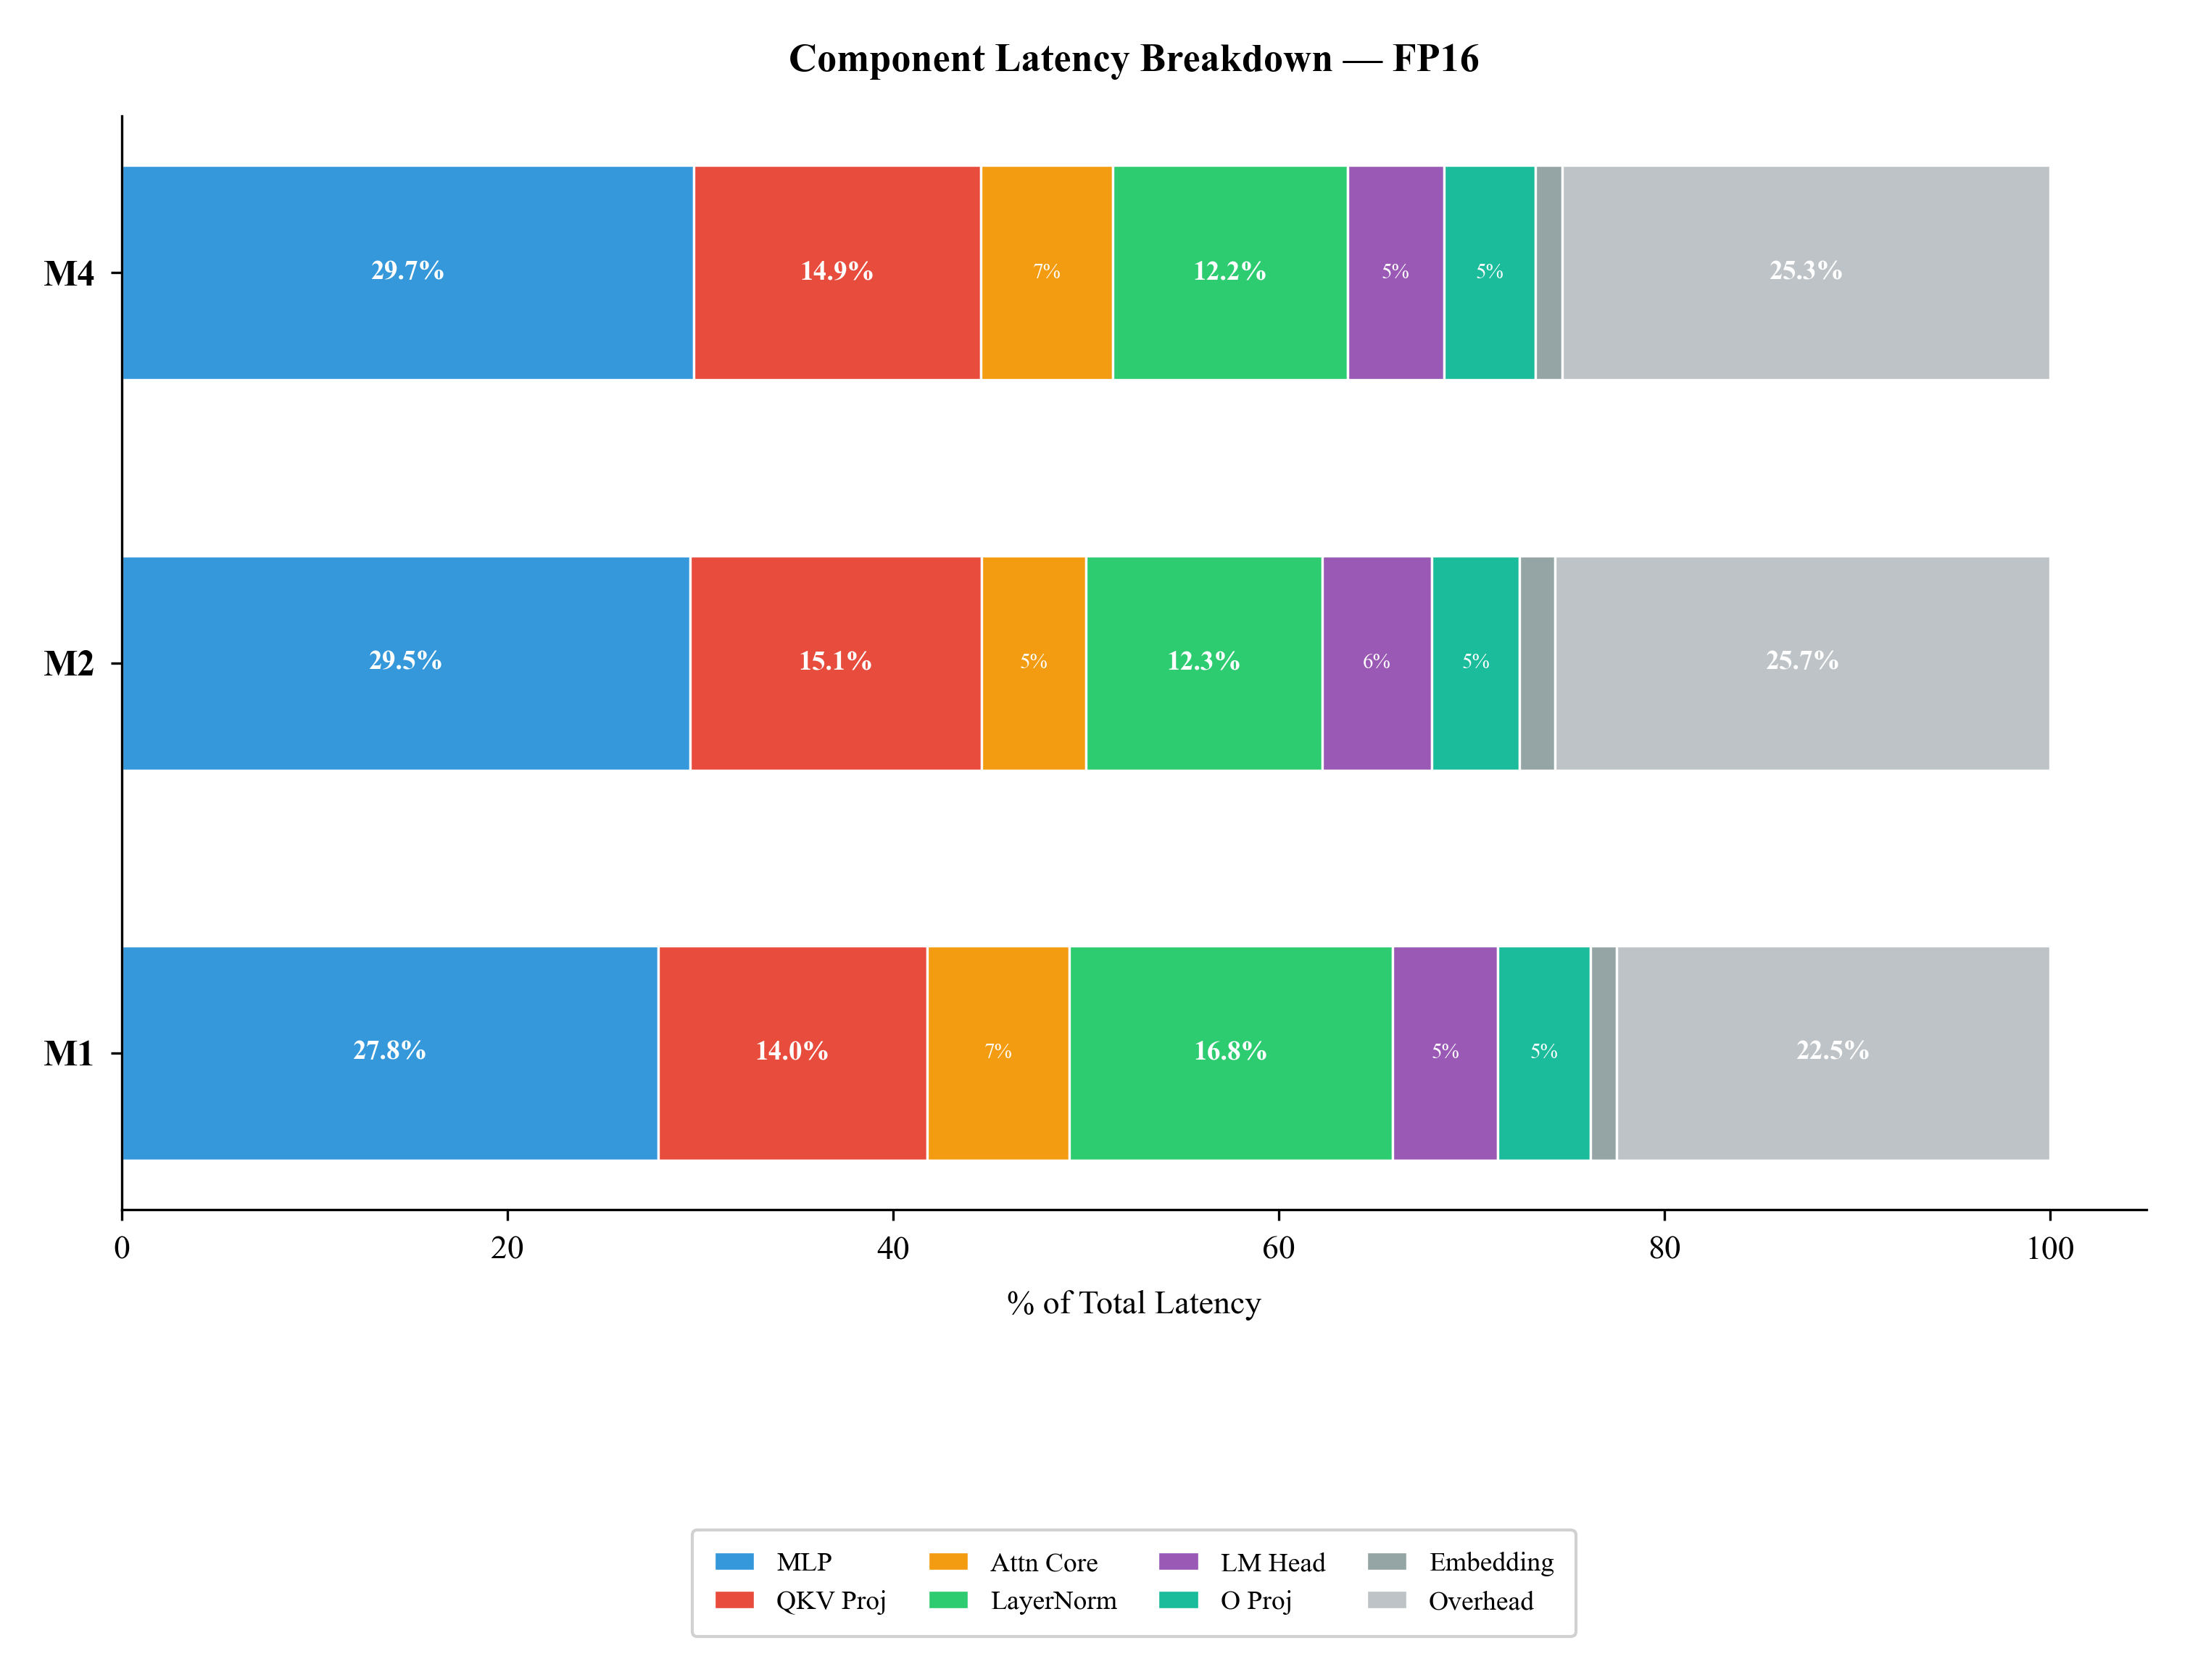
\includegraphics[width=\textwidth]{component_breakdown_f16.png}
\caption{FP16 precision}
\label{fig:decomp_f16}
\end{subfigure}
\hfill
\begin{subfigure}[b]{0.48\textwidth}
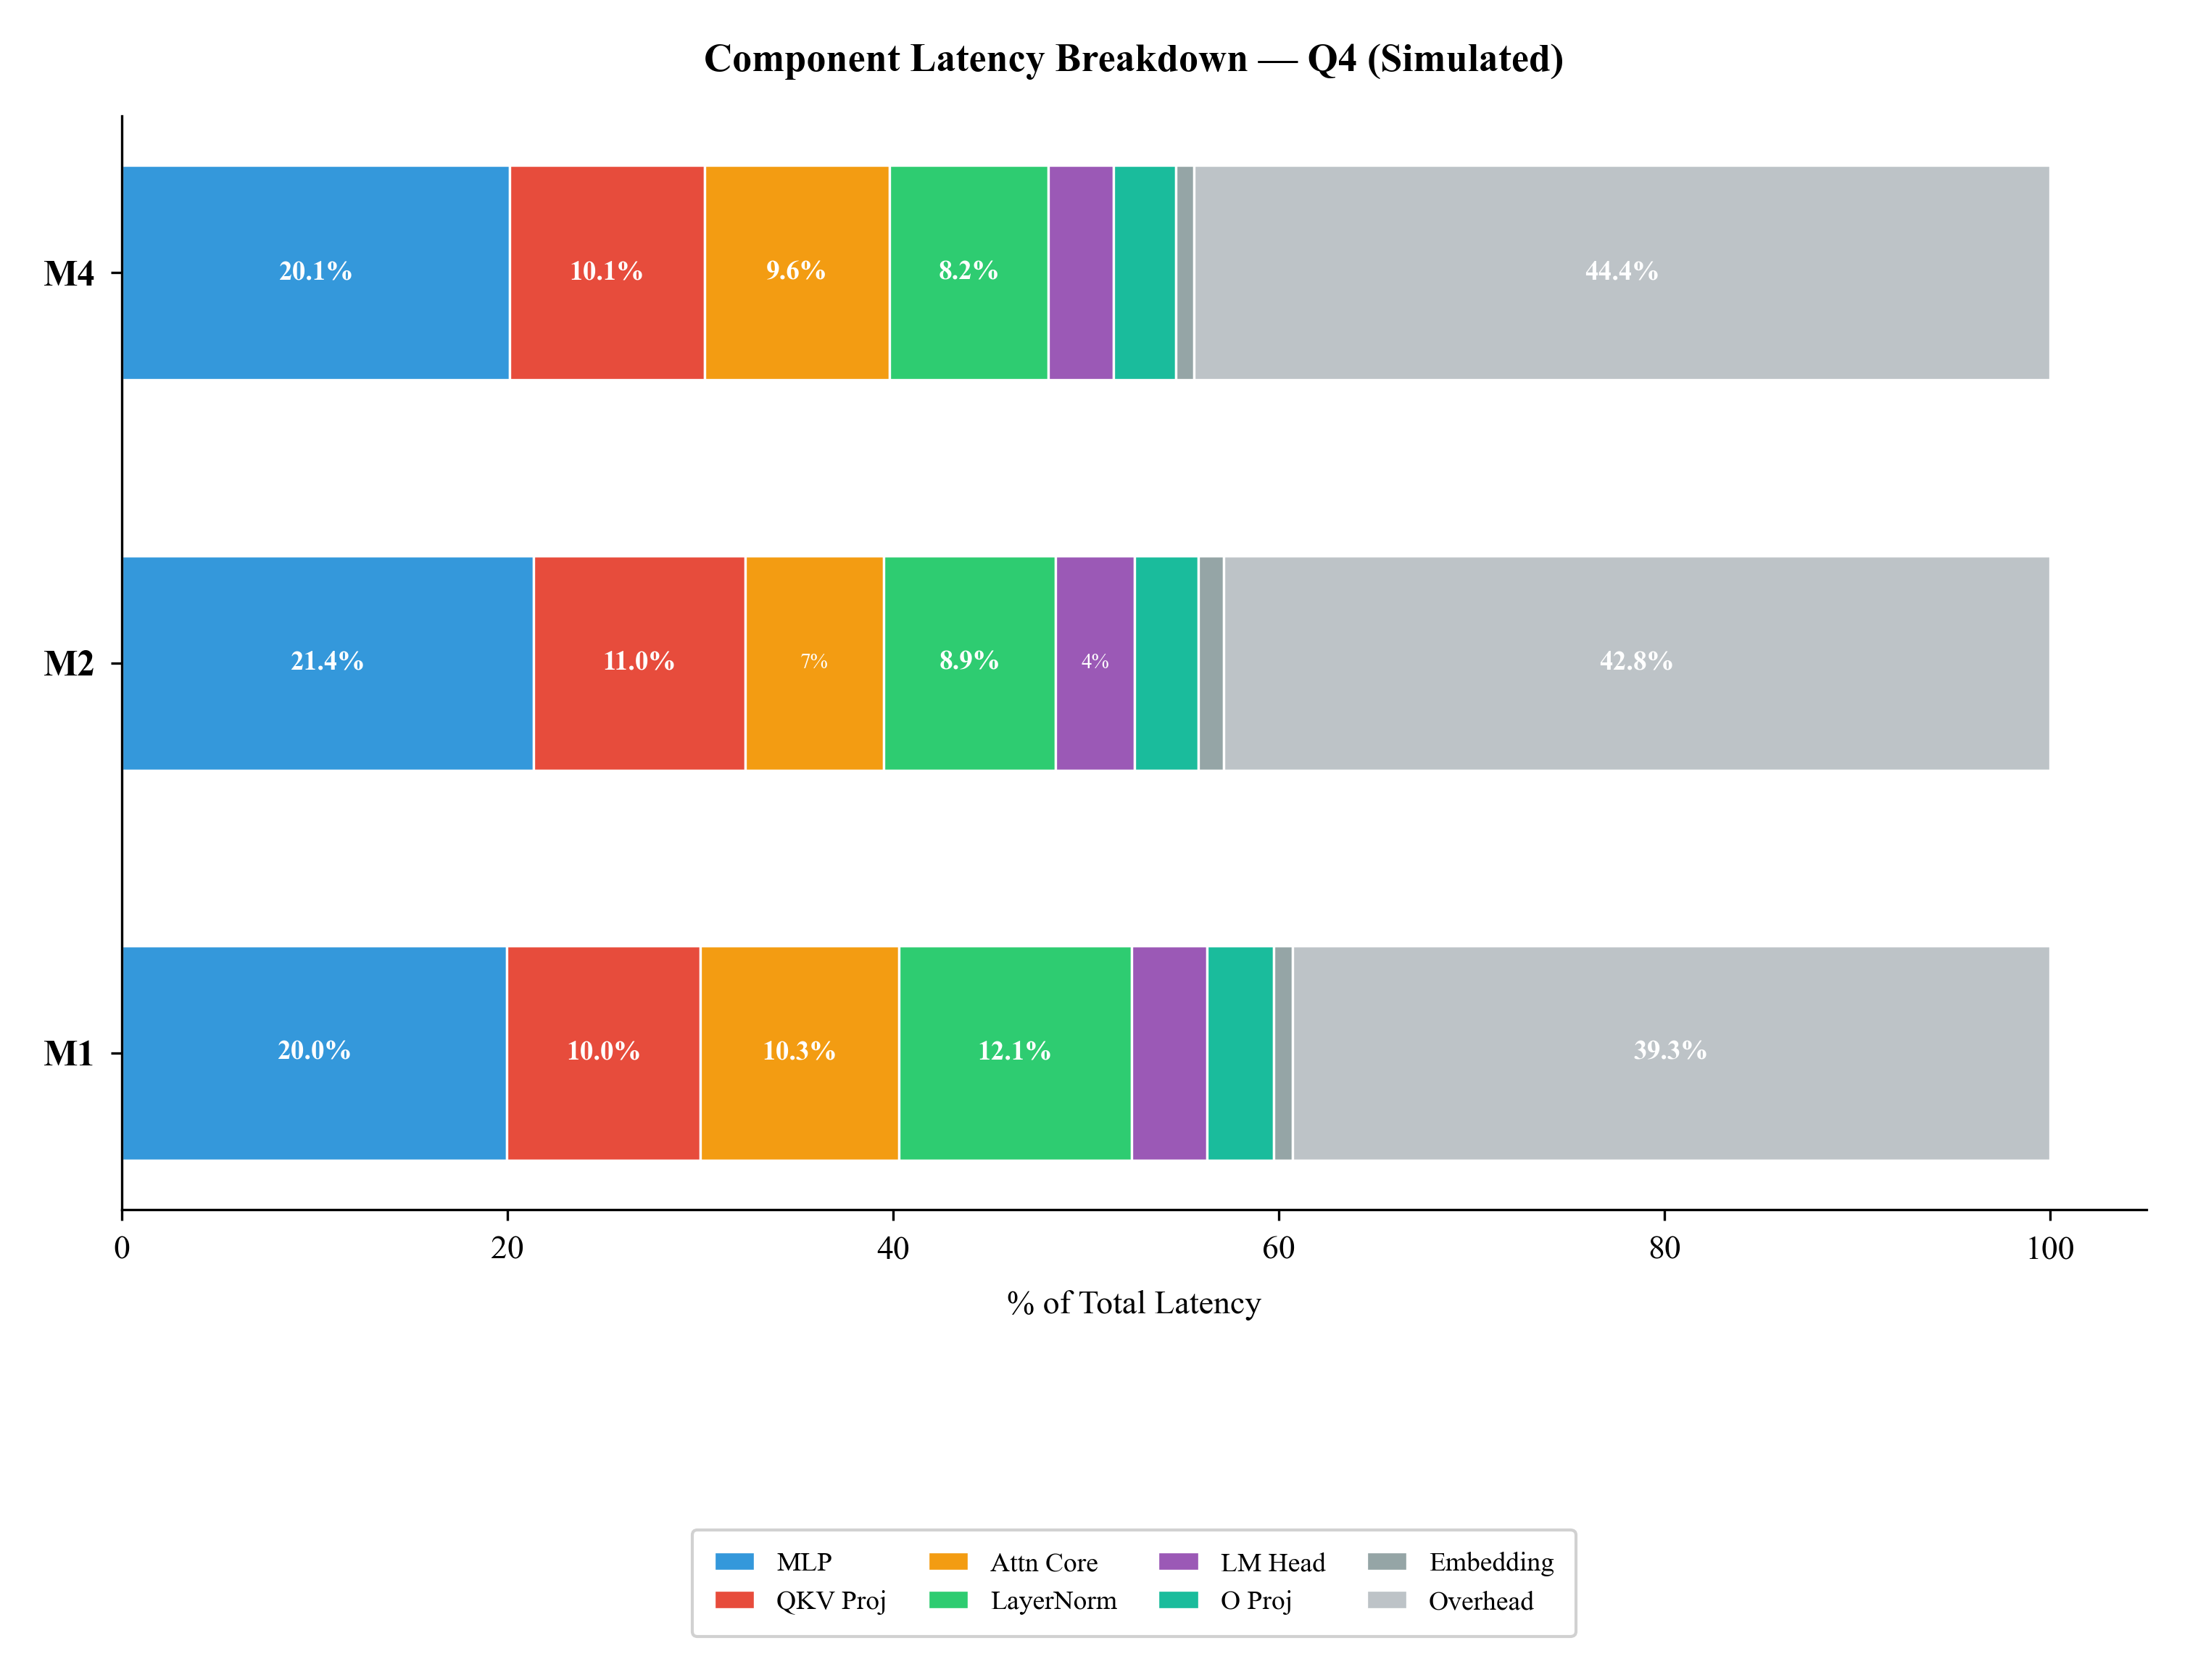
\includegraphics[width=\textwidth]{component_breakdown_q4.png}
\caption{Q4\_K\_M precision (simulated)}
\label{fig:decomp_q4}
\end{subfigure}
\caption{Per-component latency breakdown at FP16 (left) and Q4\_K\_M (right). MLP share drops from 27.8--29.7\% at FP16 to 20.0--21.4\% at Q4 as weight bytes reduce 4$\times$. Framework overhead rises from 22.5--25.7\% to 39.3--44.4\%, becoming the dominant term at Q4.}
\label{fig:decomp}
\end{figure*}

Table~\ref{tab:decomp_q4} and Fig.~\ref{fig:decomp} reveal the central finding of this study. MLP share drops from 28--30\% to 20--21\%---a ${\sim}$30\% relative reduction, less than the theoretical 4$\times$ because dequantization adds compute cost. Framework overhead \emph{rises} from 22--26\% at FP16 to 39--44\% at Q4, becoming the single largest component on all platforms. This shift is the key insight: quantization moves the bottleneck from weight streaming to framework overhead. Attention core rises slightly in relative share (5--7\% $\rightarrow$ 7--10\%) as MLP shrinks. The practical implication is that further PTL reduction at Q4 requires reducing framework overhead (kernel fusion, compiled inference graphs) rather than further weight quantization.

% ===================================================================
% VIII. ROOFLINE ANALYSIS
% ===================================================================
\section{Roofline Analysis}

\subsection{Arithmetic Intensity and Platform Rooflines}

\begin{table}[t]
\caption{Arithmetic Intensity by Component}
\label{tab:arithmetic_intensity}
\centering
\small
\begin{tabular}{lrl}
\toprule
\textbf{Component} & \textbf{AI (FLOP/byte)} & \textbf{Status} \\
\midrule
MLP (FP16)       & 1.0  & Bandwidth-bound \\
MLP (Q4)         & 4.0  & Bandwidth-bound \\
QKV Projection   & 1.0  & Bandwidth-bound \\
O Projection     & 1.0  & Bandwidth-bound \\
Attention Core   & $\sim$20  & Bandwidth-bound \\
LayerNorm        & $<$0.1  & Bandwidth-bound \\
LM Head          & 1.0  & Bandwidth-bound \\
\bottomrule
\end{tabular}
\end{table}

As shown in Fig.~\ref{fig:roofline}, all measured components fall in the bandwidth-bound region on every platform. Despite the attention core having higher arithmetic intensity (${\sim}$20\,FLOP/byte from vector dot-products over cached K/V vectors), it remains bandwidth-bound because the ridge point for all platforms exceeds 20\,FLOP/byte. The roofline plot confirms that every component operates at low utilization of peak compute---the bottleneck is purely memory bandwidth.

% Figure 6: Roofline Plot
\begin{figure}[t]
\centering
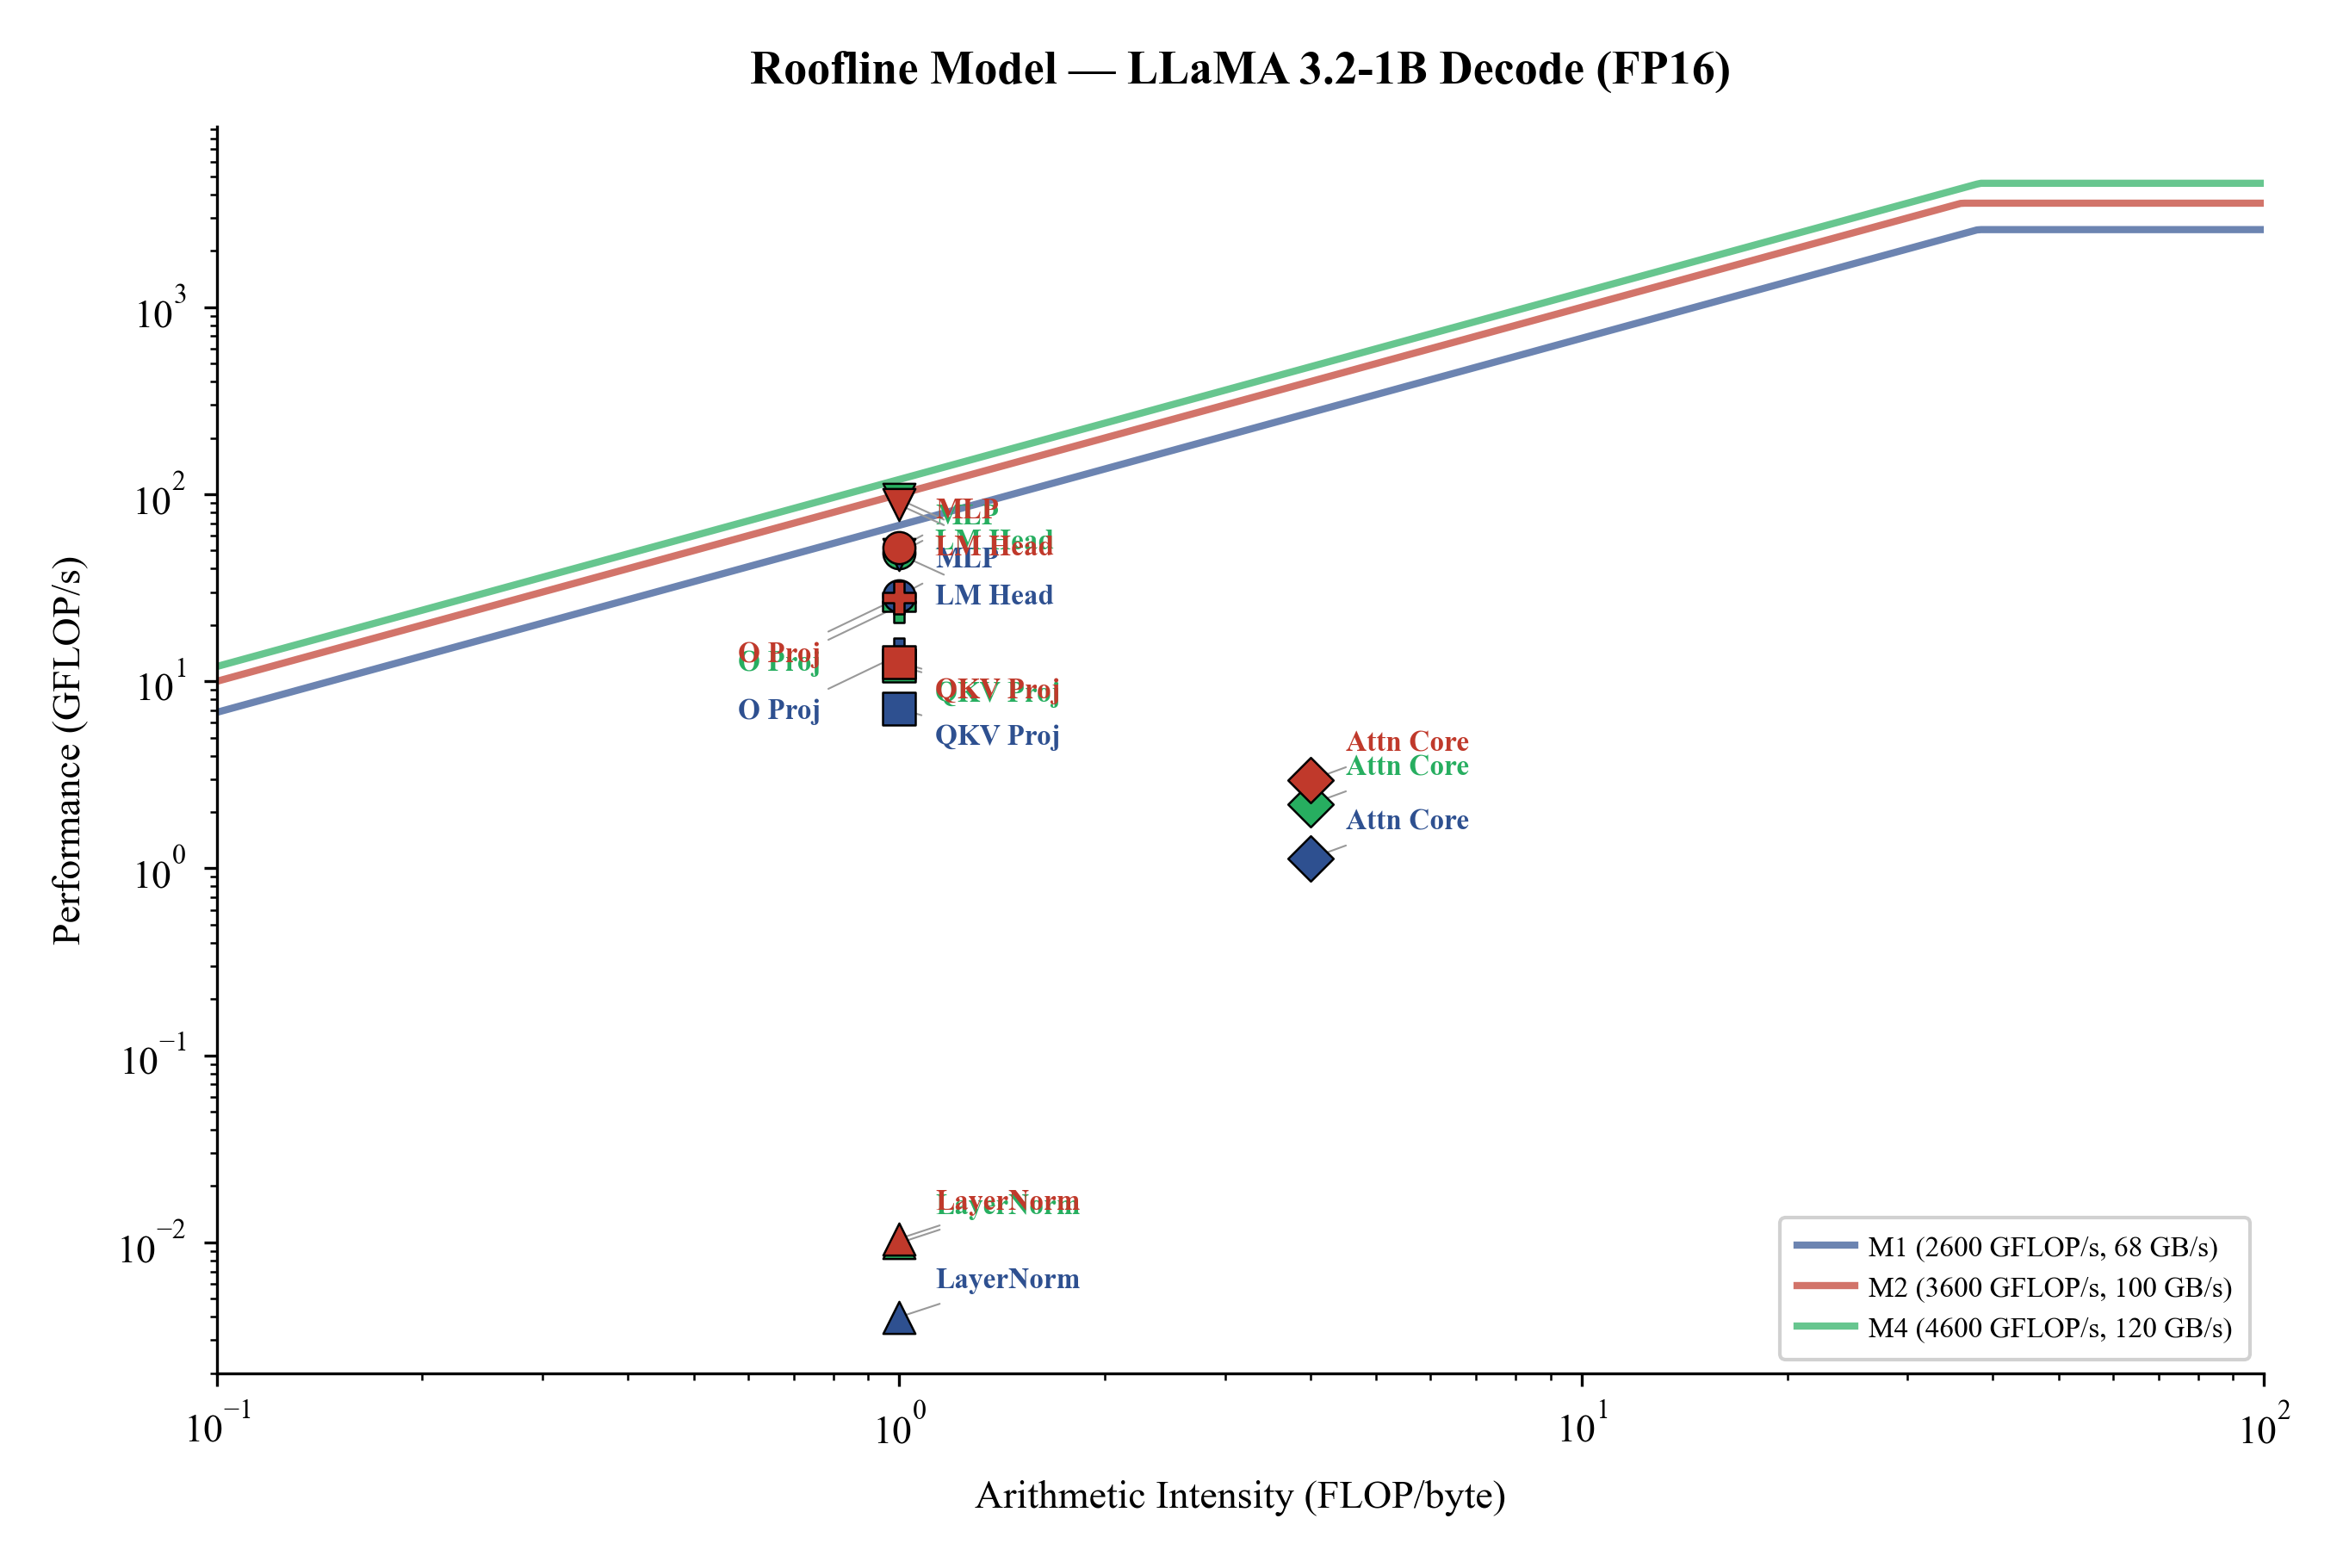
\includegraphics[width=\columnwidth]{roofline_plot.png}
\caption{Roofline model for LLaMA~3.2-1B decode at FP16. All measured components fall in the bandwidth-bound region (below each platform's ridge point). Attn Core shows higher AI due to reuse of cached K/V vectors within the attention computation.}
\label{fig:roofline}
\end{figure}

\subsection{Effective Bandwidth Utilization}

\begin{table}[t]
\caption{Effective Bandwidth Utilization (\%)}
\label{tab:bw_util}
\centering
\small
\begin{tabular}{lrrr}
\toprule
\textbf{Platform} & \textbf{FP16 (\%)} & \textbf{Q8\_0 (\%)} & \textbf{Q4\_K\_M (\%)} \\
\midrule
M1 & 85.9 & 73.0 & 52.3 \\
M2 & \textbf{89.4} & 66.4 & 51.4 \\
M4 & 81.6 & 70.7 & 52.8 \\
\bottomrule
\end{tabular}
\end{table}

As shown in Fig.~\ref{fig:bw_util}, bandwidth utilization is highest at FP16 (82--89\%) and drops with quantization (51--53\% at Q4). This is counterintuitive but explained by the overhead model: as weight bytes shrink, the fraction of step time spent in non-memory-bound operations (framework overhead, dequantization) grows, reducing the fraction of time actually streaming from DRAM. M2 shows the highest FP16 utilization (89.4\%)---the closest to its bandwidth ceiling---explaining its lower quantization speedup of 2.30$\times$.

% Figure 7: Bandwidth Utilization
\begin{figure}[t]
\centering
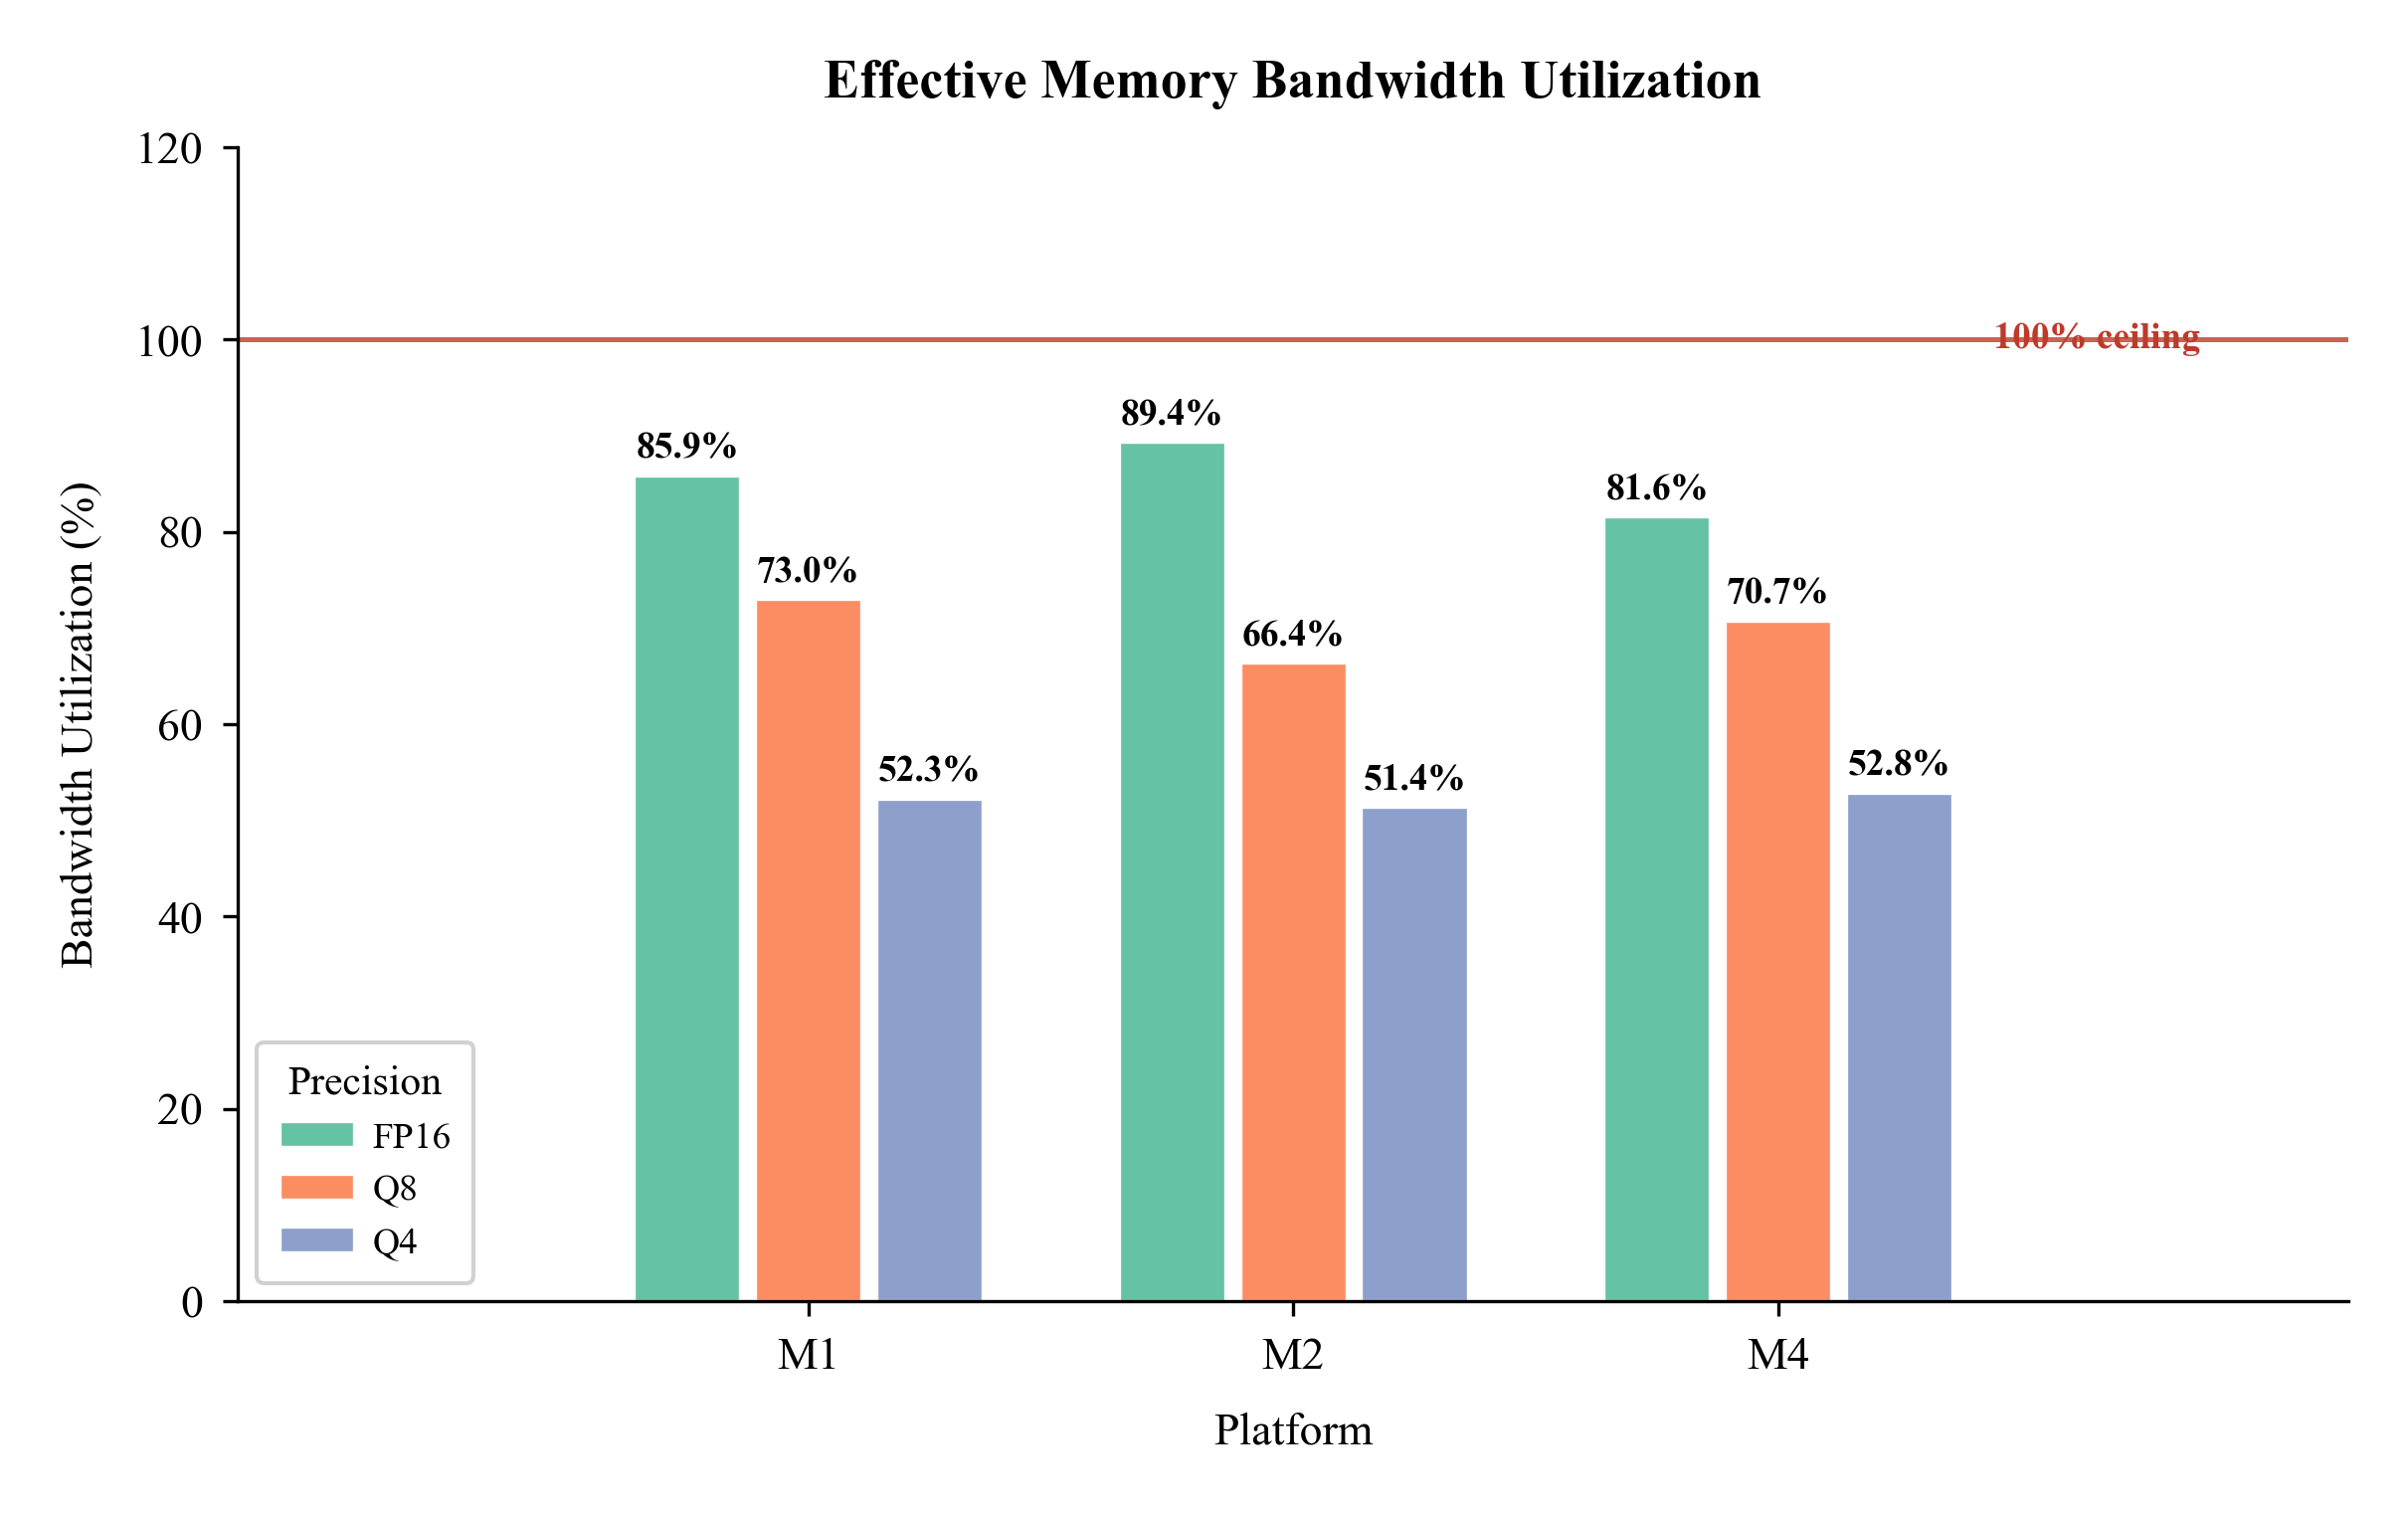
\includegraphics[width=\columnwidth]{bandwidth_utilization.png}
\caption{Effective memory bandwidth utilization per platform and precision. Utilization drops at lower precision because fixed framework overhead (dequantization, kernel launch) becomes a larger fraction of total step time, limiting effective bandwidth usage. The red dashed line marks the 100\% ceiling.}
\label{fig:bw_util}
\end{figure}

% ===================================================================
% IX. OPTIMIZATION PROPOSAL
% ===================================================================
\section{Optimization Proposal}

\begin{table}[t]
\caption{Per-Platform Optimization Roadmap}
\label{tab:roadmap}
\centering
\scriptsize
\begin{tabular}{llllc}
\toprule
\textbf{Platform} & \textbf{Bottleneck} & \textbf{Optimization} & \textbf{Est.\ $\Delta$PTL} & \textbf{Effort} \\
\midrule
M1 & Framework OH   & \texttt{torch.compile}        & 15--22\% & Med \\
M1 & KV-cache scale & INT4 KV quant                 & 12--18\% & Low \\
M2 & Framework OH   & \texttt{torch.compile}        & 14--20\% & Med \\
M2 & KV-cache scale & INT4 KV quant                 & 10--15\% & Low \\
M4 & Framework OH   & Kernel fusion + MPS graph      & 12--18\% & Med \\
M4 & Attn at long ctx & FlashAttn MPS (nightly)      & 8--14\%  & High \\
All & Context $>$512 & Sliding window attention       & 20--35\% & High \\
\bottomrule
\end{tabular}
\end{table}

Our decomposition reveals framework overhead (39--44\% at Q4) as the dominant bottleneck after quantization---not weight streaming. The most impactful optimization is therefore reducing dispatch overhead: \texttt{torch.compile} with \texttt{reduce-overhead} mode eliminates Python interpreter cost and fuses adjacent kernels, estimated to reduce the overhead component by 40--50\% and total PTL by 15--22\%. This orthogonally targets the bottleneck that quantization cannot address.

Weight quantization (Q4\_K\_M) targets the MLP and projection components but leaves KV-cache reads unchanged. At 1024-token context, KV traffic per decode step is:
\begin{equation}
  \text{KV}_{\text{bytes}} = 2 \times 32 \times 8 \times 128 \times 2 \times 1024 \approx 134\;\text{MB}
\end{equation}
INT4 KV quantization (\texttt{-ctk q4\_0} in llama.cpp) reduces this 4$\times$ to ${\sim}$33\,MB, providing orthogonal PTL reduction of 12--18\% at long contexts. Combined with \texttt{torch.compile}, the estimated total improvement is 25--38\% PTL reduction at 1024-token context on M1/M2.

% ===================================================================
% X. DISCUSSION
% ===================================================================
\section{Discussion}

\subsection{Key Findings}

\begin{enumerate}
  \item \textbf{Framework overhead dominates at Q4 precision}, rising to 39--44\% of decode time across all platforms as weight-streaming bytes shrink. This is the primary finding and explains why quantization speedup (2.30--2.59$\times$) falls well below the 4$\times$ theoretical ceiling.

  \item \textbf{MLP weight streaming remains the largest single identifiable component at FP16} (28--30\%) but is no longer dominant at Q4 (20--21\%). QKV projections follow a similar pattern (14--15\% $\rightarrow$ 10--11\%).

  \item \textbf{Bandwidth utilization paradox}: utilization is highest at FP16 (82--89\%) and lowest at Q4 (51--53\%), because quantization reduces the fraction of time spent in memory-bound operations.

  \item \textbf{PTL scaling with context length is mild at Q4} ($<$21\% growth from 64 to 1024 tokens on all platforms), suggesting Q4 is well-suited for long-context deployments where FP16 KV-cache growth would otherwise be the bottleneck.
\end{enumerate}

\subsection{Limitations}

Our study has several limitations. The forward-hook instrumentation with MPS synchronization inflates absolute per-component times by an estimated 30--40\%; however, the percentage distribution---our primary result---is reliable because the overhead applies uniformly across components. The Q4 decomposition is simulated, since llama.cpp executes quantized code paths that are not directly instrumentable via HuggingFace hooks. We benchmark only LLaMA~3.2-1B; larger models (7B+) will have different relative overhead fractions since weight-streaming cost scales with parameter count while framework overhead is more constant. Thermal throttling under sustained load was not measured and could affect reproducibility on passively cooled devices like MacBook Air. Finally, energy-per-token---a critical metric for mobile deployment---is outside the scope of this study but represents important future work.

% ===================================================================
% XI. CONCLUSION
% ===================================================================
\section{Conclusion}

We benchmarked LLaMA~3.2-1B at FP16, Q8\_0, and Q4\_K\_M across M1, M2, and M4 Apple Silicon platforms. MLP streaming dominates at FP16 (28--30\%), but framework overhead becomes the dominant term at Q4 (39--44\%) as weight bytes shrink. M4 reaches 97.2\,tok/s at Q4 with 2.59$\times$ speedup over FP16. Bandwidth utilization drops from 89\% to 51\% on M2 at lower precision, confirming that overhead---not memory limits---caps quantization gains. The primary optimization target at Q4 is therefore framework overhead reduction via \texttt{torch.compile}, not further quantization. KV-cache quantization provides complementary gains at long contexts. Apple's unified memory architecture proves well-matched to edge LLM inference, achieving high bandwidth utilization without the PCIe bottleneck present in discrete GPU systems.

% ===================================================================
% ACKNOWLEDGMENT
% ===================================================================
\section*{Acknowledgment}
The authors thank the CECS 551 course staff at California State University Long Beach for project guidance. Benchmarks were run on personal Apple Silicon hardware provided by the team members.

% ===================================================================
% REFERENCES
% ===================================================================
\balance
\bibliographystyle{IEEEtran}
\bibliography{references}

\end{document}

% ============================================================
% COMPILATION INSTRUCTIONS
% Run the following commands in the report/ directory:
%
%   pdflatex Team_7_ArchX_paper.tex
%   bibtex   Team_7_ArchX_paper
%   pdflatex Team_7_ArchX_paper.tex
%   pdflatex Team_7_ArchX_paper.tex
%
% Requires: texlive-full or equivalent with IEEEtran class
% IEEEtran.cls must be in report/ or on your LaTeX path
% ============================================================
